%%%%%%%%%%%%%%%%%%%%%%%%%%%%%%%%%%%%%%%%%
% The Legrand Orange Book
% LaTeX Template
% Version 3.1 (February 18, 2022)
%
% This template originates from:
% https://www.LaTeXTemplates.com
%
% Authors:
% Vel (vel@latextemplates.com)
% Mathias Legrand (legrand.mathias@gmail.com)
%
% License:
% CC BY-NC-SA 4.0 (https://creativecommons.org/licenses/by-nc-sa/4.0/)
%
% Compiling this template:
% This template uses biber for its bibliography and makeindex for its index.
% When you first open the template, compile it from the command line with the 
% commands below to make sure your LaTeX distribution is configured correctly:
%
% 1) pdflatex main
% 2) makeindex main.idx -s indexstyle.ist
% 3) biber main
% 4) pdflatex main x 2
%
% After this, when you wish to update the bibliography/index use the appropriate
% command above and make sure to compile with pdflatex several times 
% afterwards to propagate your changes to the document.
%
%%%%%%%%%%%%%%%%%%%%%%%%%%%%%%%%%%%%%%%%%

%----------------------------------------------------------------------------------------
%	PACKAGES AND OTHER DOCUMENT CONFIGURATIONS
%----------------------------------------------------------------------------------------

\documentclass[
	11pt, % Default font size, select one of 10pt, 11pt or 12pt
	fleqn, % Left align equations
	a4paper, % Paper size, use either 'a4paper' for A4 size or 'letterpaper' for US letter size
	%oneside, % Uncomment for oneside mode, this doesn't start new chapters and parts on odd pages (adding an empty page if required), this mode is more suitable if the book is to be read on a screen instead of printed
]{LegrandOrangeBook}

\definecolor{ocre}{RGB}{243, 102, 25} % Define the color used for highlighting throughout the book

% Book information for PDF metadata, remove/comment this block if not required 
\hypersetup{
	pdftitle={CondenC}, % Title field
	pdfauthor={Claude Jacquemard et Guillaume Laurent}, % Author field
	pdfsubject={L'essentiel des langages C et C++}, % Subject field
	pdfkeywords={C, C++}, % Keywords
	pdfcreator={LaTeX}, % Content creator field
	linkcolor=ocre
}

\addbibresource{sample.bib} % Bibliography file


\chapterimage{orange1.jpg} % Chapter heading image
\chapterspaceabove{6.5cm} % Default whitespace from the top of the page to the chapter title on chapter pages
\chapterspacebelow{6.75cm} % Default amount of vertical whitespace from the top margin to the start of the text on chapter pages

%----------------------------------------------------------------------------------------
%	FRENCH
%----------------------------------------------------------------------------------------

\usepackage[french]{babel}
\usepackage{textcomp}

\newcommand{\etc}{\emph{etc.} }
\newcommand{\cf}{\emph{cf.} }

\newenvironment{espace}{%
	\vspace{3mm}\noindent}%
	{\vspace{3mm}}


%----------------------------------------------------------------------------------------
%	LISTINGS
%----------------------------------------------------------------------------------------

\usepackage{listings}

% Cette commande permet d'utiliser �...� pour ins�rer du code en ligne, 
\lstMakeShortInline�

\lstset{language=C++,  
    basicstyle=\ttfamily,
    breaklines=true,
    columns=flexible, % pour que le code soit copiable
    keepspaces=true, % pour que le code soit copiable
    showstringspaces=false
}

\usepackage[listings,skins]{tcolorbox}
\tcbuselibrary{breakable}

\newtcblisting{cpp}{
    listing engine=listings,
    breakable,
    listing options={
        language = C++,
        breaklines=true,
        columns=flexible, % pour que le code soit copiable
        keepspaces=true, % pour que le code soit copiable
        basicstyle=\small\ttfamily,
        keywordstyle=\color{DarkBlue},
        commentstyle=\itshape\color{ForestGreen},
        showstringspaces=false
    },
    listing only,
    colback=black!5,
    left=1mm,
    top=-1mm,
    bottom=-1mm,
    frame hidden,
    enhanced,
    borderline={0.5pt}{1pt}{ocre}
}

\newtcblisting{cppsyntaxe}{
    listing engine=listings,
    breakable,
    listing options={
        language = C++,
        morekeywords = {type},
        breaklines=true,
        columns=flexible, % pour que le code soit copiable
        keepspaces=true, % pour que le code soit copiable
        basicstyle=\small\ttfamily,
        keywordstyle=\color{DarkBlue},
        commentstyle=\itshape\color{ForestGreen},
        showstringspaces=false
    },
    listing only,
    colback=green!5!white,
    left=1mm,
    top=-1mm,
    bottom=-1mm,
    frame hidden,
    enhanced,
    borderline={0.5pt}{1pt}{ocre},
}

\lstdefinelanguage{none}{
    %sensitive=false,
    %keywords={run},
    %otherkeywords={}, 
    %comment=[l]{//},
    %morecomment=[s]{/*}{*/},
    %string=[b]{"},
    %morestring=[b]{'},
    %inputencoding=latin1, % ne sert � rien ?
    %extendedchars= true,
   %mathescape=true
}

\newtcblisting{console}{
    listing engine=listings,
    breakable,
    listing options={
        language=none,
        basicstyle=\color{green}\ttfamily\small,
        frame=none,
    },
    listing only,
    colback=black,
    left=1mm,
    top=-1mm,
    bottom=-1mm,
    frame hidden,
    enhanced,
    borderline={0.5pt}{1pt}{ocre},
}


%----------------------------------------------------------------------------------------
%	TITLE PAGE
%----------------------------------------------------------------------------------------

\newcommand\HUGE{\fontsize{50}{60}\selectfont}

\begin{document}

\titlepage % Output the title page
	{
\includegraphics[width=\paperwidth]{background.pdf}} % Code to output the background image, which should be the same dimensions as the paper to fill the page entirely; leave empty for no background image
	{ % Title(s) and author(s)
		\centering\sffamily % Font styling
		{\HUGE\bfseries CondenC\par} % Book title
		\vspace{16pt} % Vertical whitespace
		{\LARGE L'essentiel des langages C et C++\par} % Subtitle
		\vspace{24pt} % Vertical whitespace
		{\huge\bfseries Claude Jacquemard et Guillaume Laurent\par} % Author name
	}

%----------------------------------------------------------------------------------------
%	COPYRIGHT PAGE
%----------------------------------------------------------------------------------------

\thispagestyle{empty} % Suppress headers and footers on this page

~\vfill % Push the text down to the bottom of the page

\noindent Copyright \copyright\ 2014 Claude Jacquemard et Guillaume Laurent\\ % Copyright notice

%\noindent \textsc{Published by Publisher}\\ % Publisher

%\noindent \textsc{\href{https://www.latextemplates.com/template/legrand-orange-book}{book-website.com}}\\ % URL

%\noindent Licensed under the Creative Commons Attribution-NonCommercial 4.0 License (the ``License''). You may not use this file except in compliance with the License. You may obtain a copy of the License at \url{https://creativecommons.org/licenses/by-nc-sa/4.0}. Unless required by applicable law or agreed to in writing, software distributed under the License is distributed on an \textsc{``as is'' basis, without warranties or conditions of any kind}, either express or implied. See the License for the specific language governing permissions and limitations under the License.\\ % License information, replace this with your own license (if any)

\noindent Cette \oe{}uvre est mise � disposition selon les termes de la licence internationale Creative Commons CC BY-NC-SA 4.0 (attribution - pas d'utilisation commerciale - partage dans les m�mes conditions).  Une copie de la licence est disponible � l'adresse \url{https://creativecommons.org/licenses/by-nc-sa/4.0}\\

%https://creativecommons.org/licenses/by-nc-sa/4.0/deed.fr

\noindent La mise en page a �t� r�alis�e avec le style \emph{The Legrand Orange Book} de Mathias Legrand disponible � l'adresse \url{https://www.latextemplates.com/template/legrand-orange-book}

%\textsc{\href{https://www.latextemplates.com/template/legrand-orange-book}{book-website.com}}\\ % URL

%\noindent \textit{First printing, March 2022} % Printing/edition date

%----------------------------------------------------------------------------------------
%	TABLE OF CONTENTS
%----------------------------------------------------------------------------------------

\pagestyle{empty} % Disable headers and footers for the following pages

\tableofcontents % Output the table of contents

%\listoffigures % Output the list of figures, comment or remove this command if not required

%\listoftables % Output the list of tables, comment or remove this command if not required

\pagestyle{fancy} % Enable default headers and footers again

\cleardoublepage % Start the following content on a new page

\noindent

%----------------------------------------------------------------------------------------
%	PART 1
%----------------------------------------------------------------------------------------

\part{Langage C}

\chapterimage{orange2.jpg} % Chapter heading image
\chapterspaceabove{6.75cm} % Whitespace from the top of the page to the chapter title on chapter pages
\chapterspacebelow{7.25cm} % Amount of vertical whitespace from the top margin to the start of the text on chapter pages

%%%%%%%%%%%%%%%%%%%%%%%%%%%%%%%%%%%%%%%%%%%%%%%%%%%%%%%%%%%%%%%%%%%%%
\chapter{Langage C}

C est un langage de programmation imp�ratif, g�n�raliste et de bas niveau invent� au cours de l'ann�e 1972 par Dennis Ritchie et Ken Thompson dans les Laboratoires Bell en m�me temps qu'Unix.\medskip

C est con�u pour �tre compil� en un nombre d'instructions machine assez pr�visible en termes d'occupation m�moire et de charge de calcul. Il utilise des types entiers et flottants correspondant aux types de donn�e support�s par le processeur et permet la gestion directe de la m�moire par l'interm�diaire de pointeurs.\medskip

Ce document propose un condens� de la syntaxe du langage illustr� de nombreux exemples. 

%%%%%%%%%%%%%%%%%%%%%%%%%%%%%%%%%%%%%%%%%%%%%%%%%%%%%%%%%%%%%%%%%%%%%
\section{Symboles, identificateurs et commentaires}

%--------------------------------------------------------------------
\subsection{Symboles de base du langage}\index{symboles}\index{caract�res sp�ciaux}

Lettres~: �A, ..., Z, a, ..., z�

Chiffres~: �0, ..., 9�

Caract�res sp�ciaux~: \lstinline�+ - * / _ = < > ^ ~ ( ) [ ] { } .,; : ' " \ | & % ! ?� et l'espace.

%--------------------------------------------------------------------
\subsection{Identificateurs}\index{identificateurs}

Un identificateur commence par une lettre ou �_�, suivi d'une
combinaison de lettres, de chiffres et �_� (l'espace et autres
symboles sp�ciaux sont proscrits).

\medskip
Le langage C distingue les majuscules des minuscules dans les identificateurs.

\begin{remark}
Pour nommer les variables et les fonctions, il est d'usage d'utiliser le �snake_case� ou le �camelCase� avec des caract�res minuscules.
\end{remark}
\begin{remark}
Il est d'usage d'utiliser  le �SCREAMING_SNAKE_CASE� avec des caract�res majuscules pour nommer les constantes et les macro-instructions.
\end{remark}

\newpage

%--------------------------------------------------------------------
\subsection{Mots r�serv�s}\index{mots}\index{mots r�serv�s}

Un certain nombre d'identificateurs sont r�serv�s et ne peuvent �tre red�finis
par l'utilisateur ou utilis�s autrement que suivant la syntaxe pr�vue. Les mots r�serv�s du C sont :

\begin{cppsyntaxe}                      
auto      do        goto      signed    unsigned
break     double    if        sizeof    void
case      else      int       static    volatile
char      enum      long      struct    while
const     extern    register  switch
continue  float     return    typedef
default   for       short     union
\end{cppsyntaxe}


%--------------------------------------------------------------------
\subsection{Commentaires}\index{commentaires}

Un commentaire dans un programme C se place entre les balises �/*� et �*/� et peut se prolonger sur plusieurs lignes.

\begin{cpp}
/* ceci est un commentaire */
\end{cpp}

%%%%%%%%%%%%%%%%%%%%%%%%%%%%%%%%%%%%%%%%%%%%%%%%%%%%%%%%%%%%%%%%%%%%%
\section{Types simples}

%--------------------------------------------------------------------
\subsection{Type �num�r�}\index{types!�num�r�s}\index{enum}

Un type �num�r� est d�fini par l'�num�ration ordonn�e des identificateurs
repr�sentant les constantes du type, entre accolades.

\begin{cppsyntaxe}
enum identificateur_de_type { LISTE_DES_CONSTANTES };
\end{cppsyntaxe}

Les �l�ments de la liste sont s�par�s par des virgules.

\begin{cpp}
enum couleur { TREFLE, CARREAU, COEUR, PIQUE };
  /* TREFLE est cod� par la valeur 0, CARREAU par la valeur 1, etc. */

enum jour { LUNDI=1, MARDI, MERCREDI, JEUDI, VENDREDI, SAMEDI };
  /* LUNDI est cod� par la valeur 1, MARDI par la valeur 2, etc. */

enum booleen { FAUX=0, VRAI=1 };
\end{cpp}



%--------------------------------------------------------------------
\subsection{Type entier~: char, short, int, long, unsigned}\index{entiers}\index{types!entiers}

La diff�rence entre les diff�rents types entiers est uniquement sur le nombre d'octets
de codage en m�moire~:
\begin{remark}
\begin{tabular}{ll}
    \lstinline�char�  & entier sur 1 octet (-128 � 127)\index{char}\\
    \lstinline�short� & entier sur 2 octets (-32\,768  �  32\,767)\index{short}\\
    \lstinline�int�   & entier sur 2 ou 4 octets suivant les compilateurs et les
    processeurs\index{int}\\
    \lstinline�long�  & entier sur 4 octets (-2\,147\,483\,648 �
    2\,147\,483\,647)\index{long}\\
    \lstinline�long int� & �quivalent � \lstinline�long�\\
\end{tabular}
\end{remark}


Tous ces types entiers peuvent �tre pr�c�d�s du mot-cl� �unsigned�.
\index{unsigned}
\begin{remark}
\begin{tabular}{ll}
    \lstinline�unsigned char�  & entier sur 1 octet (0 � 255)\\
    \lstinline�unsigned short� & entier sur 2 octets (0 � 32\,767)\\
    \lstinline�unsigned int�   & entier sur 2 ou 4 octets suivant les compilateurs et les processeurs\\
    \lstinline�unsigned long�  & entier sur 4 octets (0 � 4\,294\,967\,295)\\
\end{tabular}
\end{remark}


\subsection{Type r�el~: float, double}\index{r�els}\index{types!r�els}

La repr�sentation flottante utilise une mantisse et un exposant cod�s sur un certain nombre
d'octets.

\begin{remark}
\begin{tabular}{ll}
    \lstinline�float� & r�el sur 4 octets (de 3,4e-38 � 1,7e38 avec 7 chiffres
    significatifs)\index{float}\\
    \lstinline�double� & r�el sur 8 octets (de 1,7e-308 � 3,4e308 avec 15 chiffres
    significatifs)\index{double}\\
    \lstinline�long double� & r�el sur 10 octets (de 3,4e-4932 � 1,7e4932 avec 18 chiffres
    significatifs)\index{long double}\\
\end{tabular}\end{remark}

%--------------------------------------------------------------------
\subsection{Type vide~: void}\index{void}\index{types!vide}

Le type �void� est un type de taille m�moire nulle.

%--------------------------------------------------------------------
\subsection{Type pointeur}\index{pointeurs}\index{types!pointeurs}

Un pointeur (adresse) est typ� par le type de l'objet point�, pr�c�d� de *.

\begin{cpp}
int *pe;   /* pe est un pointeur sur un entier */
char *pc;  /* pc est un pointeur sur un caract�re */
\end{cpp}

Il existe une constante de type pointeur pr�-d�finie dans les biblioth�ques standards, la constante �NULL�.\medskip

Un pointeur du type �void *� n'est pas typ� et est g�n�rique.

%--------------------------------------------------------------------
\subsection{Autres types}\index{cha�nes de caract�res}\index{bool�ens}\index{types!bool�ens}\index{types!cha�nes de caract�res}

Le langage C ne fournit pas d'autres types, notamment pas de type bool�en ni de type
cha�ne. N�anmoins, une cha�ne de caract�re est habituellement stock�e dans un tableau de caract�res (\cf~\ref{sec:chaine}).

%--------------------------------------------------------------------
\subsection{Conversion de type (cast)}\index{conversion de type}\index{cast}\index{types!conversions}

En plus des r�gles standards de conversion de type dans les expressions, les
identificateurs de type peuvent servir d'op�rateurs de conversion.

\begin{cpp}
float x;
int i;
i=(int) x;
\end{cpp}

%--------------------------------------------------------------------
\subsection{Autres types}\index{cha�nes de caract�res}\index{bool�ens}\index{types!bool�ens}\index{types!cha�nes de caract�res}

Le langage C ne fournit pas d'autres types, notamment pas de type bool�en ni de type
cha�ne. N�anmoins, une cha�ne de caract�re est habituellement stock�e dans un tableau de caract�res (\cf~\ref{sec:chaine}).

\pagebreak

%%%%%%%%%%%%%%%%%%%%%%%%%%%%%%%%%%%%%%%%%%%%%%%%%%%%%%%%%%%%%%%%%%%%%
\section{Constantes, variables et expressions}

%--------------------------------------------------------------------
\subsection{Constantes}\index{constantes}\index{const}

Le mot r�serv� �const� permet de d�clarer des constantes.

\begin{cppsyntaxe}
const type NOM = valeur;
\end{cppsyntaxe}

Exemple :
\begin{cpp}
const float PI = 3.14159;
const char CR = '\n';
\end{cpp}


Le langage C utilise les conventions ci-dessous pour coder des valeurs constantes :

\begin{remark}
\begin{tabular}{lllll}
d�cimal~:     & \lstinline�2�     & \lstinline�-12�   & \lstinline�+123�    &         \\
octal~:       & \lstinline�012�   & \lstinline�03775� &           & (pr�c�d� de 0)    \\
hexad�cimal~: & \lstinline�0xa�   & \lstinline�0XA1F� &           & (pr�c�d� de  0x ou 0X)    \\
non sign�~:   & \lstinline�12u�   & \lstinline�012u�  & \lstinline�0xa1fu�  & (entier suivi de u)  \\
entier long~: & \lstinline�12l�   & \lstinline�012L�  & \lstinline�0xa1fuL� & (entier suivi de l ou L)  \\
\\
r�el~:        & \lstinline�2.�    & \lstinline�3.14�  & \lstinline�-45.2�   & �.15�   \\
              & \lstinline�2.25f� & \lstinline�3.01F� &                     & (virgule fixe~: f ou F) \\
              & \lstinline�10e-1� & \multicolumn{2}{l}{\lstinline�-45.2E+12�} & (virgule flottante~: e ou E) \\
\\
caract�re~:   & \lstinline�'a'�   & \lstinline�'C'�   &  \lstinline�'+'�     & (entre simples quotes)  \\
\\
cha�ne~:     & \multicolumn{2}{l}{\lstinline�"commentaire"�} & \lstinline�"Claude"� & (entre doubles quotes)   \\
\end{tabular}
\end{remark}


Les caract�res sp�ciaux sont pr�c�d�s d'un \lstinline�\� (anti-slash ou
contre-barre).\index{caract�res sp�ciaux}


\begin{remark}
\begin{tabular}{ll}
    \lstinline�'\n'�   &    nouvelle ligne \\
    \lstinline�'\r'�   &    d�but de ligne \\
    \lstinline�'\b'�   &    retour arri�re \\
    \lstinline�'\t'�   &    tabulation   \\
    \lstinline�'\medskip'�   &    contre-barre  \\
    \lstinline�'\f'�   &    nouvelle page \\
    \lstinline�'\0'�   &    caract�re \lstinline�NULL�  \\
    \lstinline�'\''�   &    simple quote    \\
    \lstinline�'\"'�   &    double quote    \\
    \lstinline�'\ooo'� &    caract�re de code octal ooo  \\
    \lstinline�'\xhh'� &    caract�re de code hexad�cimal hh  \\
\end{tabular}
\end{remark}


%--------------------------------------------------------------------
\subsection{Variables}\index{variables}

Toute variable doit �tre d�clar�e avant sa premi�re utilisation. Une
initialisation peut �tre faite au moment des d�clarations.

\begin{cppsyntaxe}
type liste_de_noms_de_variables;

type noms = valeurs;
\end{cppsyntaxe}

Exemple :
\begin{cpp}
char a, b;
int j, i = 2;
float resultat = 0.0;
char nombre = '1',  lettre = 'a';
\end{cpp}


%--------------------------------------------------------------------
\subsection{Op�rateurs arithm�tiques}\index{op�rateurs!arithm�tiques}

Op�rateurs binaires~:\index{+} \index{-} \index{*}\index{/} \index{\%}

\begin{remark}
\begin{tabular}{ll}
    \lstinline�+� &  addition\index{additions}\\
    \lstinline�-� &  soustraction\index{soustractions}\\
    \lstinline�*� &  multiplication\index{multiplications}\\
  \lstinline�/� &  division (enti�re si les deux op�randes sont entiers, r�elle sinon)\index{divisions}\index{divisions!enti�res} \\
    \lstinline�%� &  modulo (reste de la division enti�re )\index{modulo}\\ 
\end{tabular}
\end{remark}


Op�rateurs unaires~: \index{++} \index{--}

\begin{remark}
\begin{tabular}{ll}
    \lstinline�-� &  oppos�\\
    \lstinline�++� & auto-incr�mentation (pr� ou post-fixe)\index{incr�mentation}\\
    \lstinline�--� &  auto-d�cr�mentation (pr� ou post-fixe)\\
\end{tabular}
\end{remark}

Exemples d'utilisation :
\begin{cpp}
int i = 1, j, k;
j = i++;    /* j re�oit la valeur 1, puis i est modifi� en 2 */
k = ++j;    /* j est d'abord modifi�e en 2, puis k re�oit 2 */
i++;        /* i est modifi� en 3 */
\end{cpp}

%--------------------------------------------------------------------
\subsection{Op�rateurs relationnels}\index{op�rateurs!relationnels}\index{comparaisons} \index{<} \index{>}\index{<=} \index{>=}\index{==}\index{"!=}

Ils permettent de comparer deux op�randes. Le r�sultat de la comparaison est un nombre entier~: 0 si le r�sultat est faux, 1 si le r�sultat est vrai.

\begin{remark}
\begin{tabular}{ll}
               \lstinline�<�  &  inf�riorit� stricte\index{inf�riorit�}\\
                \lstinline�>�  &  sup�riorit� stricte\index{sup�riorit�}\\
                \lstinline�<=� &  inf�riorit� large    \\
                \lstinline�>=� &  sup�riorit� large    \\
                \lstinline�==� &  �galit�\index{�galit�}\\
                \lstinline�!=� &  in�galit�\index{in�galit�}\index{diff�rence}\\
\end{tabular}
\end{remark}

Exemple d'utilisation :
\begin{cpp}
int b;
b = ( x != y );  /* b re�oit la valeur 0 si x est �gal � y, 1 sinon */
\end{cpp}


%--------------------------------------------------------------------
\subsection{Op�rateurs logiques}\index{op�rateurs!logiques}\index{"!} \index{\&\&}\index{\textbar{}\textbar{}}

Comme pour les op�rateurs relationnels, le r�sultat d'une expression logique est une valeur enti�re 0 ou 1.

\begin{remark}
\begin{tabular}{ll}
    \lstinline�!� &  n�gation logique\index{non!logique}\\
    \lstinline�&&� & et logique\index{et!logique}\\
    \lstinline�||� & ou logique\index{ou!logique}\\
\end{tabular}
\end{remark}

Exemple:
\begin{cpp}
c = (a || b) && (i < j);
\end{cpp}


Remarques:
\begin{itemize}
    \item dans l'expression �(A&&B)�, si �A� est faux, �B� n'est pas �valu�
  \item dans l'expression �(A||B)�, si �A� est vrai, �B� n'est pas �valu�
\end{itemize}


%--------------------------------------------------------------------
\subsection{Op�rateurs sur les bits}\index{op�rateurs!bits}\index{\&}\index{\textbar{}} \index{\^\ } \index{\~\ }\index{op�rateurs!d�calages}\index{d�calages}

Ils ne peuvent �tre employ�s que sur des op�randes entiers et op�rent bit � bit.

\begin{remark}
\begin{tabular}{ll}
    \lstinline�&� & et\index{et!bits}\\
    \lstinline�|� & ou\index{ou!bits}\\
    \lstinline�^� & ou exclusif\index{ou exclusif!bits}\\
    \lstinline�~� & n�gation (compl�ment)\index{non!bits}\\
    \lstinline�<<� & d�calage � gauche\\
    \lstinline�>>� & d�calage �  droite\\
\end{tabular}
\end{remark}

Exemple:
\begin{cpp}
y = x << 3;  /* y re�oit la valeur de x d�cal�e de 3 bits vers la gauche (correspond � x multipli� par 2 puissance 3), cod� sur le m�me nombre de bits que x. */
\end{cpp}

%--------------------------------------------------------------------
\subsection{Op�rateurs d'affectation}\index{op�rateurs!affectations}\index{affectations}

L'affectation est consid�r�e comme un op�rateur.

\begin{cppsyntaxe}
var = expr /* o� var est une variable et expr une expression. */
\end{cppsyntaxe}

Lors d'une affectation comme �x = expression�, l'expression est �valu�e, cette valeur est affect�e � la variable �x�, de plus, cette valeur est le r�sultat de l'op�ration d'affectation. \medskip

Ceci permet des affectations multiples en une seule instruction comme �x = y = z = 1�    (�z� re�oit 1, le r�sultat de l'affectation qui est 1 est affect� � �y�, \etc).\medskip

Ceci permet �galement les affectations compos�es. Ces affectations combinent les op�rateurs arithm�tiques, logiques et de d�calage avec l'affectation.\index{op�rateurs!affectations~compos�es}
\index{affectations!compos�es}

\begin{cppsyntaxe}
var op= expr /* o� var est une variable, expr une expression 
                et op= un op�rateur. */
\end{cppsyntaxe}

Ceci est �quivalent � �v = (v) op (e)�     

\begin{remark}
\begin{tabular}{ll}
Arithm�tiques & \lstinline�+=      -=      *=      /=      %=�\\ 
Logiques      & \lstinline�&=      |=      ^=�\\
D�calage      & \lstinline�<<=      >>=�\\  
\end{tabular}
\end{remark}



Exemples:
\begin{cpp}
x += 1     /* correspond � x = x+1  ou �  x++  */
a *= b      /* correspond �  a = a*b  */
h &= xFF /* correspond �  h = h & xFF  */
r <<= 4     /* correspond �  r = r << 4  */
\end{cpp}

%--------------------------------------------------------------------
\subsection{Op�rateur conditionnel ?}\index{op�rateurs!conditionnel}
\index{affectations!conditionnelles} \index{?} 

L'op�rateur conditionnel �?� est un op�rateur ternaire. 

\begin{cppsyntaxe}
e1 ? e2 : e3 
\end{cppsyntaxe}

Si �e1� est vrai, l'expression est �gale � la valeur �e2�, sinon l'expression est �gale � �e3�. Par exemple:
\begin{cpp}
m = ( a > b ) ? a : b;  /* m re�oit le max de a et b */
( a == b ) ? c++ : c--; /* on ajoute 1 � c si a est �gale � b, sinon on enl�ve 1 � c */
\end{cpp}

\begin{remark}
L'op�rateur conditionnel �tant tr�s peu lisible, il est recommand� de l'utiliser avec parcimonie...
\end{remark} 

%--------------------------------------------------------------------
\subsection{Op�rateur de taille (sizeof)}\index{op�rateurs!de taille}\index{sizeof}

Cet op�rateur d�livre le nombre d'octets occup�s en m�moire par une expression ou un type. La valeur retourn�e est du type �size_t� (entier non sign�). Pour un type, des parenth�ses sont requises, car il s'agit alors d'une fonction.

\begin{cpp}
int a;
int b[100];

n = sizeof a;   /* utile pour conna�tre la taille des entiers */
n = sizeof b / sizeof b[0];    /* permet de conna�tre la nombre d'�l�ments du tableau b */
\end{cpp}

%--------------------------------------------------------------------
\subsection{Op�rateurs sur les pointeurs}\index{op�rateurs!pointeurs}\index{pointeurs!op�rateurs}

Il existe quelques op�rateurs unaires sur les pointeurs :

\begin{remark}
\begin{tabular}{ll}
    \lstinline�*�  & donne acc�s � l'�l�ment point�\\
    \lstinline�&�  & fournit l'adresse de la variable\\
    \lstinline�++� & incr�mente le pointeur du nombre d'octets de l'objet point�\\
  \lstinline�--� & d�cr�mente le pointeur du nombre d'octets de l'objet point�
\end{tabular}
\end{remark}

Exemples d'utilisation:
\begin{cpp}
int  e = 0;
int *pe;  /* pe est un pointeur sur un entier */
pe = &e;  /* pe re�oit l'adresse de la variable enti�re e */
*pe = 3;  /* l'emplacement point� par pe re�oit 3 */
pe++;     /* pe pointe 2 octets plus loin */
*pe = 4;
\end{cpp}

Les fonctions �malloc()� et  �free()� de la biblioth�que standard permettent d'allouer et de lib�rer dynamiquement de la m�moire. \index{allocations}\index{malloc}\index{free}
Elles retournent des pointeurs du type �void *�, c'est-�-dire des pointeurs non typ�s. Le pointeur retourn� par �malloc()� peut �tre converti en pointeur typ�.\medskip

S'il n'y a plus de place m�moire disponible, la fonction �malloc� retourne la valeur �NULL�.

\begin{cpp}
char  *p;   /* p est un pointeur sur un caract�re */
p = malloc(100); /* alloue de la place pour 100 caract�res */
...
free(p);    /* lib�re la place des 100 caract�res */
        
truc *q;    /* q est un pointeur sur un type truc d�fini ailleurs*/    
q = (truc *)malloc(10*sizeof(truc));
            /* alloue de la place pour 10 �l�ments de type truc  */
\end{cpp}

%--------------------------------------------------------------------
\subsection{Op�rateur de s�quence}\index{op�rateurs!de s�quence}

L'op�rateur de s�quence (\lstinline�,�) autorise une liste d'expressions l� o� une seule expression est permise. Dans ce cas, les expressions sont �valu�es de gauche vers droite. Le type et la valeur de la liste d'expressions est donc le type et la valeur de l'expression la plus � droite.

\begin{cpp}
for ( i=0,j=0; i<10; i++,j++ ) 
    ...
\end{cpp}

%--------------------------------------------------------------------
\subsection{Priorit� des op�rateurs}\index{op�rateurs!priorit�s}\index{priorit�s des op�rateurs}

%En l'absence de parenth�ses, l'ordre de priorit� des op�rateurs de C et C++ est consign� dans le tableau en annexe \ref{chap:priorite}.

Les op�rateurs sont class�s du plus prioritaire (niveau 16) au moins prioritaire (niveau 1).

\begin{center}
\small
\begin{tabular}{|l|l|l|}
\hline
	\textbf{Niveau}	& \textbf{Op�rateur} & \textbf{Descriptif} \\ \hline
	
  %17 & \lstinline$::$	         &	op�rateur de port�e globale \\
    % & \lstinline$::$	         &	op�rateur de port�e de la classe \\ \hline 

  16 & \lstinline$->   . $     &	s�lection d'un membre de structure\\
     & \lstinline$[ ]$	       &  indexation de tableau\\
     & \lstinline$( )$         &	appel d'une fonction\\
     & \lstinline$sizeof$	     &	taille en octets\\ \hline 
	
  15 & \lstinline$++   -- $    &  auto incr�mentation et d�cr�mentation\\
     & \lstinline$~  !$           & 	n�gation bit � bit	et n�gation logique\\
%		 & \lstinline$!$           &	n�gation logique \\
		 & \lstinline$+   - $	     &  plus et moins unaires \\
		 & \lstinline$* $          &	acc�s � une variable point�e\\
		 & \lstinline$&$           &  adresse d'une variable\\
		 & \lstinline$( )$         &  conversion de type\\
%		 & \lstinline$new  delete$ &	op�rateurs de gestion m�moire\\ \hline 

	14 & \lstinline$->*   .*$		 &  s�lection d'un membre de structure\\ \hline 

	13 & \lstinline$*   /   %$	 &	op�rateurs multiplicatifs\\ \hline 

	12 & \lstinline$+   -$			 &  op�rateurs additifs\\ \hline 

	11 & \lstinline$>>   <<$		 &  op�rateurs de d�calage\\ \hline 

	10 & \lstinline$<   <=   >   >=$	& op�rateurs de relation\\ \hline 

	9	 & \lstinline$==   !=$	   &	�galit� et in�galit�\\ \hline 

	8	 & \lstinline$&	$         &  et bit � bit\\ \hline 

	7	 & \lstinline$^$	         &	ou exclusif bit � bit\\ \hline 

	6	 & \lstinline$|$	         &  ou bit � bit\\ \hline 

	5	 & \lstinline$&&$	         &  et logique\\ \hline 

	4	 & \lstinline$||$          &  ou logique\\ \hline 

	3	 & \lstinline$? :$         & op�rateur conditionnel\\ \hline 

	2  & \lstinline$=   *=   /=   %=   +=   -=$	& op�rateurs d'affectation\\
		 & \lstinline$<<=   >>=   &=   ^=   |=$	 &	et d'affectation compos�e\\ \hline 

	1	&	\lstinline$,$			       & op�rateur de s�quence\\ \hline
\end{tabular}
\end{center}



%%%%%%%%%%%%%%%%%%%%%%%%%%%%%%%%%%%%%%%%%%%%%%%%%%%%%%%%%%%%%%%%%%%%%
\section{Types compos�s}\index{types!compos�s}

%--------------------------------------------------------------------
\subsection{D�finition de type~: typedef}\index{types!d�finition}\index{typedef}

L'instruction �typedef� permet de nommer un nouveau type ou renommer
un type existant.

\begin{cppsyntaxe}
typedef description_du_type identificateur_de_type;
\end{cppsyntaxe}

Exemple:
\begin{cpp}
typedef short petit_entier; /* petit_entier d�signera un short */
typedef short booleen; /* booleen d�signera aussi un short */
typedef char chaine[20]; /* chaine est le nom du type tableau de 20 caract�res */
\end{cpp}

Le langage C fournit une seule structure de donn�es, le tableau et permet la construction de nouveaux types structur�s (�struct� et �union�).
    
%--------------------------------------------------------------------
\subsection{Tableaux}\index{tableaux}


\subsubsection{Tableaux mono-dimensionnels}\index{tableaux!mono-dimensionnels}

Un tableau est une collection d'�l�ments du m�me type accessibles par un indice.


\begin{cppsyntaxe}
type nom[taille];    
\end{cppsyntaxe}


o�:
\begin{itemize}
    \item �taille� est une expression constante enti�re,
    \item les �l�ments du tableau sont accessibles par un indice compris entre 0 et taille-1;
\end{itemize}
 
\begin{cpp}
int a[10]; /* d�clare une variable tableau a de 10 �l�ments a[0], ..., a[9] */
typedef char message[20]; /* message est le nom du type tableau de 20 caract�res */
typedef float tab[10]; /* tab est le nom du type tableau de 10 r�els */
\end{cpp}
 
\begin{remark}
En g�n�ral, le compilateur ne v�rifie pas les d�bordements d'indice!
\end{remark}

Un tableau peut �tre initialis� lors de sa d�claration par une liste de valeurs entre accolades (si la liste est insuffisante, la fin du tableau est initialis�e par des 0).

\begin{cpp}
char alerte[10] = { 'A', 't', 't', 'e', 'n', 't', 'i', 'o', 'n', '!' };
float a[] = { 1.0, 2.0, -3.14 }; /* r�serve la place pour un tableau de 3 r�els */
int b[5] = { 1, 2, 3 }; /* b[3] et b[4] sont mis � 0 */
\end{cpp}


\subsubsection{Relations entre tableaux et pointeurs}\index{tableaux!pointeurs}

En C, l'identificateur d'une variable tableau est �quivalent � un pointeur constant pointant sur le premier �l�ment du tableau.

\begin{cpp}
int a[10];  
int *pa;
pa = a; /*  Le pointeur sur entier pa contient l'adresse de l'entier a[0],
            i.e l'adresse du d�but du tableau a.  */
pa = &a[0]; /* c'est �quivalent */
\end{cpp}

Ainsi, �a[0]� est accessible par �*pa�, c'est-�-dire par \lstinline�*(&a[0])�.\medskip

D'autre part, un pointeur peut s'auto-incr�menter. L'adresse contenue dans le pointeur est automatiquement augment�e du nombre d'octets du type de l'�l�ment point�. De fa�on g�n�rale, �a[i]�  est accessible par  �*(pa+i)�. Les instructions suivantes sont donc �quivalentes: �a[1]=x;�, �*(pa+1)=x;� et �*(++pa)=x;�, par exemple :

\begin{cpp}
/* trois fa�ons �quivalentes de traiter le tableau a.*/
for (i=0; i<10; i++) a[i]    = i;        
for (i=0; i<10; i++) *(pa+i) = i;
for (i=0; i<10; i++) *(pa++) = i;
\end{cpp}

\og{}�quivalent\fg{} signifie ici que le r�sultat est identique pour l'utilisateur externe; ce n'est �videmment pas identique pour la machine et ses performances.\medskip

\begin{remark}
Ne pas oublier que le nom du tableau est une adresse constante. Par cons�quent, des instructions comme \lstinline�a++� ou \lstinline�a = pa� sont ill�gales si $a$ est un tableau.
\end{remark}
        
\subsubsection{Tableaux multi-dimensionnels}\index{tableaux:multi-dimensionnels}


\begin{cppsyntaxe}
type nom[taille1][taille2]...[taillen];
\end{cppsyntaxe}

Exemple:

\begin{cpp}
int a[5][3];    
/* a est un tableau de 5 lignes et 3 colonnes, a[i][j]  0<=i<=4, 0<=j<=2 */
/* a est un tableau de 5 �l�ments, chaque �l�ment a[i] �tant un tableau de 3 entiers */
\end{cpp}
     
Les �l�ments sont stock�s en m�moire de fa�on contigu�.

Un tableau peut �tre initialis� lors de sa d�claration par une liste de valeurs entre accolades.

\begin{cpp}
int a[3][2] = { 1,2,3,4,5,6 }; /* vision mono-dimensionnelle */
int a[3][2] = { {1,2},{3,4},{5,6}}; /* vision multi-dimensionnelle */
\end{cpp}

De par la relation entre tableau et pointeur, �a[i]� est aussi un pointeur et �a� un pointeur sur pointeur. Les notations suivantes sont donc �quivalentes : 
\begin{enumerate}
    \item notation indic�e habituelle:    �a[i][j]�,
    \item vision du tableau bidimensionnel comme tableau de pointeurs: �*(a[i]+j)�,
    \item vision du tableau bidimensionnel comme pointeur de pointeur: �*(*(a+i)+j)�,
    \item vision du tableau bidimensionnel comme tableau monodimensionnel: �*(*a+ i*m+j)� soit �*(&a[0][0]+ i*m+j)�. 
\end{enumerate}

\subsubsection{Allocation dynamique de tableaux}\index{tableaux:allocation dynamique}\index{allocations:tableaux}\index{malloc}
    
\begin{cpp}
int *pa;
pa = ( int *)malloc(100); /* est une fa�on d'allouer dynamiquement un tableau de 100 entiers */

char *chaine;
chaine = malloc(30); /*    est une fa�on d'allouer dynamiquement un tableau de 30 caract�res, soit une cha�ne de 30 caract�res. */

truc *ptruc; /* o� le type truc  est d�fini par ailleurs */
ptruc = (truc *)malloc(10*sizeof(truc)); 
ptruc = malloc(10*sizeof(truc)); 
/* sont des fa�ons d'allouer dynamiquement un tableau de 10 trucs. */
\end{cpp}

%--------------------------------------------------------------------
\subsection{Cha�nes de caract�res}\label{sec:chaine}\index{cha�nes de caract�res}  

En langage C, une cha�ne de caract�res est habituellement d�fini par un tableau de caract�res. Le dernier caract�re d'une cha�ne est le caract�re sp�cial �'\0'�.

\begin{cpp}
char a[10] = "Claude";
char b[10] = { 'C','l','a','u','d','e','\0' }; 
a[2]='o';  
a[3]='\0'; /* a contient alors la cha�ne "Clo" */

char a[] = "Claude"; /* r�serve la place suffisante pour la cha�ne, soit ici un tableau de 7 caract�res */ 
\end{cpp}

Le type chaine n'est pas pr�d�fini, il est utile de le d�finir:
\begin{cppsyntaxe}
typedef char chaine[30];
/* d�claration du type cha�ne de 30 caract�res, num�rot�s de 0 � 29, seuls 29 caract�res sont utilisables � cause du caract�re de fin */
\end{cppsyntaxe}



L'affectation d'une cha�ne � une valeur ne peut se faire en utilisant l'op�rateur �=�, car il y aurait copie d'adresse uniquement et de plus, un tableau est un pointeur constant. L'affectation est donc r�alis� � l'aide du sous-programme �strcpy� de la biblioth�que standard.

\index{affectations!cha�nes de caract�res}\index{strcpy} 
     
\begin{cpp}
char a[10];
strcpy(a,"Crac"); /* a = "Crac" est impossible */

typedef char couleur[10];
couleur drapeau[3];
/* drapeau  est un tableau de 3 pointeurs sur des caract�res */
        
strcpy(drapeau[0], "bleu");
strcpy(drapeau[1], "blanc");
strcpy(drapeau[2], "rouge");

/* ou */
char *drapeau[3] = { "bleu","blanc","rouge" };
\end{cpp}

D'autres sous-programmes (comparaison, concat�nation, \etc) de manipulation de cha�nes de caract�res sont disponibles dans la biblioth�que standard �string.h�  (\cf~\ref{sec:string.h}).

%--------------------------------------------------------------------
\subsection{Structures}\index{structures}\index{enregistrement}\index{struct}

\subsubsection{D�finition}

Le mot r�serv� �struct� permet de d�finir son propre type structur� compos� de champs. Une structure est commun�ment appel�e \emph{enregistrement}.

\begin{cppsyntaxe}
struct nom_de_la_structure { d�clarations_des_champs; };
\end{cppsyntaxe}

Exemples:

\begin{cpp}
struct complexe {
         float x,y; };
         
struct complexe a,b; /* a et b sont deux variables de type complexe */

struct date { 
        char jour[10];
        char mois[12];    
        int annee; }  d1, d2; /* d1 et d2 sont deux variables de type date */
\end{cpp}

Pour �viter de r�p�ter le mot �struct� lors de la d�claration des variables, on peut d�finir un nouveau type � l'aide de �typedef�:

\begin{cpp}
typedef struct { 
          int dim; 
          float t[30]; } vecteur;

vecteur v;

typedef struct {
          int jour;
          char mois[12];
          int  annee; } date;
          
date d;
          
typedef struct {
          char nom[20],prenom[20];
          date date_de_naissance; } individu;

individu  moi, lui, classe[30];

/* moi et lui  sont deux variables de type individu, classe un tableau de 30 individus */
\end{cpp}

On peut d�finir des structures r�cursives ou auto-r�f�renc�es en utilisant typedef.

\begin{cpp}
typedef struct { 
            individu valeur; 
            struct noeud *fils_droit;
            struct noeud *fils_gauche; } noeud;

noeud  *arbre; /* arbre est une variable pointeur sur un noeud  */
\end{cpp}

\subsubsection{Affectation et initialisation}\index{affectations!structures}

L'affectation s'effectue globalement sur tous les membres des structures.
\begin{cpp}
d1 = d2;
moi = lui;
\end{cpp}

On peut aussi initialiser une structure lors de sa d�claration :
\begin{cpp}
individu toto = {"Dupond","Pierre",{12,"Mars",1975}};
\end{cpp}

\subsubsection{Acc�s aux champs}\index{champs}\index{.}

L'acc�s aux champs se fait par l'ajout d'un point apr�s l'identificateur suivi du nom du champ.

\begin{cpp}
v.dim=2;
v.t[2]=12;

a.x=0;
a.y=1; /* a est le complexe 0+i */ 

d={30,"Mars",1976};
 
moi.date_de_naissance=d;
lui.date_de_naissance.jour=4;
classe[1].date_de_naissance.annee=1985;
\end{cpp}

\begin{remark}
L'acc�s aux champs d'une structure point�e peut �tre simplifi� par la notation �->� : �X->Y� signifie �(*X).Y� soit le champ �Y� de la structure point�e par �X�. \index{->}
\end{remark}

\begin{cpp}
individu *toto;        /* toto est un pointeur sur un individu */
toto=malloc(sizeof(individu));
toto->date_de_naissance.annee=1996
/* �quivalent � :  (*toto).date_de_naissance.annee = 1996 */
\end{cpp}


%--------------------------------------------------------------------
\subsection{Unions}\index{unions}\index{union}

Le mot r�serv� �union� permet de d�finir des variables pouvant contenir des valeurs de types diff�rents.

\begin{cpp}
typedef union {
          struct { int x,y; } cartesien;
          struct { float rho,teta; } polaire;
          } complexe;

complexe a;
\end{cpp}

Un complexe peut contenir soit une structure de deux entiers, soit une structure de deux r�els.

Ainsi, les notations suivantes sont licites :    �a�, �a.cartesien�,  �a.cartesien.x�, �a.cartesien.y�, �a.polaire�, �a.polaire.rho�, �a.polaire.teta�.

\begin{cpp}
typedef enum { CERCLE = 1, RECTANGLE } type_dessin;
    
typedef struct { 
          type_dessin  figure;
          union {   
            struct { float centre_x,centre_y,rayon; } cercle; 
            struct { float centre_x,centre_y,longueur,largeur;} rectangle;
            } primitive_dessin;
          } objet_graphique;

objet_graphique c,r;    
\end{cpp}

On peut donc �crire: �c.figure�, �c.primitive_dessin�, �c.primitive_dessin.cercle�, 

�c.primitive_dessin.cercle.rayon�, �r.figure�, �r.primitive_dessin�, 

�r.primitive_dessin.rectangle�, �r.primitive_dessin.rectangle.largeur�.

%%%%%%%%%%%%%%%%%%%%%%%%%%%%%%%%%%%%%%%%%%%%%%%%%%%%%%%%%%%%%%%%%%%%%
\section{Structures de contr�le}\index{structures de contr�le}

%--------------------------------------------------------------------
\subsection{Blocs et port�e des d�clarations}\index{blocs}\index{port�e}

Une instruction est une expression suivie d'un point-virgule.

\begin{cpp}
i=1;
k++;
l=produit(a,b);
\end{cpp}

Un bloc est une suite d'instructions entre deux accolades. Les instructions sont ex�cut�es en s�quence, dans l'ordre de leur �criture. Un bloc est une instruction compos�e. Par cons�quent, partout o� une instruction est licite, on peut placer un bloc.

\begin{cpp}
{
  i=1;
  k++;
  l=produit(a,b);
}
\end{cpp}

Une variable peut �tre d�clar�e dans n'importe quel bloc, sous les conditions suivantes :
\begin{itemize}
    \item elle doit �tre d�clar�e avant toute instruction du bloc,
    \item sa port�e (son existence) est limit�e au bloc o� elle est d�clar�e.
\end{itemize}

Elle est alors connue et accessible dans le bloc et les blocs embo�t�s.

\begin{cpp}
{ 
  int i; 
  i=1; 
  ..
  { 
    float k=0;
    k=i+1; /* ici i est accessible */
    ...
  }
  i=2;  /* ici k n'est pas accessible */
  ...
  { 
    int i=10;    /* on a ici un i propre au bloc embo�t� */
    ...
  }
  /* on retrouve ici le i du bloc englobant qui vaut 2 */     
} 
\end{cpp}




%--------------------------------------------------------------------
\subsection{Instructions de choix~: if, switch}

\subsubsection{Instruction if}\index{if}\index{else}\index{structures de contr�le!si alors sinon}\index{si alors sinon}


\begin{cppsyntaxe}
if (expression)
    instruction1;
else 
    instruction2;
\end{cppsyntaxe}



L'expression peut �tre de type entier, �num�r�, r�el ou pointeur. L'instruction 1 est ex�cut�e si l'expression a une valeur non nulle, l'instruction 2 est ex�cut�e si l'expression a une valeur nulle.\medskip

La partie �else� est facultative.

\begin{cpp}
if (i==j)
  i++;
  
if (a>b)
  max=a; 
else 
  max=b;
  
if ((a>b)&&(i>j)) { 
  a=i; 
  b=j;
} else { 
  a=j;
  b=i; 
}
\end{cpp}

\subsubsection{Instruction switch}\index{switch}\index{structures de contr�le!choix multiples}

C'est une instruction � choix multiples. Elle permet de remplacer des s�quences ou des cascades de �si�.


\begin{cppsyntaxe}
switch ( expression ) {
    case constante1 : instructions1;
    case constante2 : instructions2;
    ...
    case constanten : instructionsn;
    default         : instructions;
}
\end{cppsyntaxe}


        
L'expression doit �tre de type entier ou �num�r�. Le type des constantes doit �tre le m�me que celui de l'expression.\medskip

Suivant la valeur de l'expression, le branchement s'effectue au cas correspondant et \emph{tout} ce qui suit est ex�cut� jusqu'� la rencontre d'un �break�.\index{break} Si aucune constante n'est �gale � l'expression, le branchement se fait sur �default�. Ce cas �default� est facultatif.

\begin{cpp}
char c; 
int i=0,j=0,k=0; 
...
switch (c) {
  case 'a' : i=1; 
  case 'b' : j=1; 
  case 'c' : k=1; break;
  case 'q' : j=2; break;
  default  : k=2;
}  
\end{cpp}

On peut grouper plusieurs constantes, comme dans l'exemple suivant :

\begin{cpp}
int i,k; 
...
switch ( i%6 ) {
  case 0 : k++; break;
  case 1 :  
  case 2 : k--; break;
  case 3 : 
  case 4 : 
  case 5 : k*=2; break;
}  
\end{cpp}

%--------------------------------------------------------------------
\subsection{Instructions d'it�rations : while, do, for}

\subsubsection{Instruction while}\index{while}\index{structures de contr�le!tant que}\index{tant que}


\begin{cppsyntaxe}
while (expression)
    instruction;
\end{cppsyntaxe}



L'instruction est ex�cut�e tant que l'expression a une valeur non nulle.        

\begin{cpp}
int compteur=0;
while (compteur<10) {   
  ...
  compteur++; 
}
\end{cpp}

\subsubsection{Instruction do}\index{do}\index{structures de contr�le!r�p�ter}\index{r�p�ter}


\begin{cppsyntaxe}
do
    instruction;
while (expression);
\end{cppsyntaxe}



Contrairement au �while�, l'instruction est ex�cut�e avant la premi�re �valuation de l'expression.
  
\begin{cpp}
s=0;
i=1;
do {
  s+=a[i]*b[i]; 
  i++;
} 
while (i<=10);
\end{cpp}
        
\subsubsection{Instruction for}\index{for}\index{structures de contr�le!pour}\index{pour}

\begin{cppsyntaxe}
for (expression1; expression2; expression3)
    instruction;
\end{cppsyntaxe}

L'instruction �for� est �quivalente � :     
\begin{cpp}
expression1;
while (expression2) { 
    instruction;
    expression3
};
\end{cpp}

Exemples: 
\begin{cpp}
s=0;  
for (i=1;i<=n;i++) 
  s+=a[i]*b[i];

for (i=0;i<10;i++) {
  if (a[i]) {
    k=0; 
  }
  a[i]=i; 
}
\end{cpp}

Une boucle �for� peut utiliser une variable de type �num�r�e. De plus, les expressions et l'instruction peuvent �tre vides, c'est-�-dire omises (mais les points-virgules restent !).
\begin{cpp}
s=0;  
i=1; 
for (;  i<=n; i++)
  s+=a[i]*b[i];

s=0;  
for (i=1; i<=n; ) { 
  s+=a[i]*b[i];
  i++;
}

for (s=0, i=1; i<=n; s+= [i]*b[i], i++) ;
\end{cpp}


                                 
%--------------------------------------------------------------------
\subsection{Instructions de ruptures de s�quence}\index{rupture de s�quence}
 
\subsubsection{Instruction goto}\index{goto}

Toute instruction peut �tre pr�c�d�e d'une �tiquette (suivie de : ) � laquelle peut se r�f�rer une instruction �goto�.
L'�tiquette et les �goto� s'y r�f�rant doivent appartenir � la m�me fonction.

\begin{cpp}
i=1;  
... 
if (k==i) 
  goto ailleurs;
...  
ailleurs : i=2; 
...
\end{cpp}

\begin{remark}
L'instruction �goto� est h�rit�e des instructions de saut des langages machines mais il est recommand� de ne plus l'utiliser depuis les ann�es 70... 
\end{remark}

\subsubsection{Instruction break}\index{break}

L'instruction �break� permet de sortir d'une it�ration �while�, �do�, �for� ou d'une instruction de choix multiple �switch�.
 
\begin{cpp}
s=0;
for (i=1;; i++) { 
  if (i>n) 
    break; 
  s+=a[i]*b[i]; 
}
/* le break est le seul moyen de sortir d'une telle boucle */
\end{cpp}

\begin{remark}
L'instruction �break� introduit une rupture dans la s�quence qui peut conduire � des traitements inachev�s, il convient donc de l'utiliser avec parcimonie.
\end{remark}

L'instruction �continue� permet d'ignorer le reste des instructions du corps de l'it�ration et � passer directement � l'it�ration suivante.\index{continue}

\begin{cpp}
s=0;
for (i=1; i<=n; i++)
{
  if (s>max)
    break;
  else
    s+=a[i];
}

i=0; 
s=0;
while (i<=n+1) { 
  i++;
  if (i%2) 
    continue;  
  s+=a[i]; 
}
\end{cpp}

\subsubsection{Instruction exit}\index{exit}\label{sec:exit}

La fonction �void exit(int valeur);� termine l'ex�cution du programme. Elle peut se placer n'importe o� dans le programme ou dans une fonction.

Par convention, une valeur nulle (on peut aussi utiliser la constante nulle �EXIT_SUCCESS�) signifie que le programme s'est termin� normalement, une valeur non nulle signifie que le programme s'est termin� avec une erreur (constante �EXIT_FAILURE�).

%%%%%%%%%%%%%%%%%%%%%%%%%%%%%%%%%%%%%%%%%%%%%%%%%%%%%%%%%%%%%%%%%%%%%
\section{Fonctions}\index{fonctions}\index{sous-programme}

%--------------------------------------------------------------------
\subsection{En-t�te d'une fonction (ou signature, ou prototype)}\index{protoptype}\index{en-t�te}\index{signature}\index{fonction!en-t�te}


\begin{cppsyntaxe}
type nom_de_la_fonction ( liste_de_param�tres_formels );
\end{cppsyntaxe}



Les param�tres de la liste sont s�par�s par des virgules.
La liste des param�tres peut �tre vide (�void�).\medskip

Une fonction retourne une valeur du type indiqu�. Si le type de la fonction n'est pas pr�cis�, la fonction est par d�faut de type �int�.\medskip

Une fonction peut ne rien retourner (proc�dure); elle sera alors d�clar�e de type �void�.\index{proc�dures}

\begin{cpp}
int puissance (int x, int y);
/* retourne l'entier x puissance y */

void message_d_alerte(void);
/* ne retourne rien */

complexe *add_complexe(complexe a, complexe b);
/* retourne un pointeur sur le r�sultat complexe a+b */
\end{cpp}

Le nom des arguments est facultatif dans les prototypes de fonctions; les types suffisent.

\begin{cpp}
int puissance(int,int);

complexe *add_complexe(complexe,complexe);
\end{cpp}

L'en-t�te d'une fonction peut �tre plac�e avant son utilisation, la fonction elle-m�me pouvant alors �tre d�crite en dehors du programme ou dans un autre fichier.

%--------------------------------------------------------------------
\subsection{D�finition d'une fonction (corps)}\index{d�finition}\index{corps}\index{fonction!d�finition}


\begin{cppsyntaxe}
type  nom_de_la_fonction ( liste_de_param�tres_formels ) {
    d�clarations;
    instructions;
    return ...;
}
\end{cppsyntaxe}

La valeur retourn�e se fait par l'instruction �return� qui provoque ensuite la sortie de la fonction.

\begin{cppsyntaxe}
return expression;
\end{cppsyntaxe}

Les fonctions peuvent naturellement �tre r�cursives.

\begin{cpp}
int puissance(int x, int y) {
    int   i, r  = 1;
    for (i=1; i<=y; i++) 
        r*=x;
    return r;    
} /* retourne x puissance y */

typedef struct { float  x, y; }  complexe;

complexe sous_complexe(complexe a, complexe b) 
{   complexe   r;
    r.x = a.x-b.x;   r.y = a.y-b.y;
    return r; 
} /* retourne le r�sultat complexe a-b */

complexe   *add_complexe ( complexe a, complexe b ) 
{   complexe  *r;
    r=malloc(sizeof(complexe));
    r->x = a.x+b.x;   r->y = a.y+b.y;
    return r; 
} /* retourne un pointeur sur le r�sultat complexe a+b */

\end{cpp}

%--------------------------------------------------------------------
\subsection{Passage des param�tres}\index{param�tres}\index{passage!par valeur}
\label{sec:passage_des_param�tres}

En C, le seul type de passage de param�tres est le passage par valeur.
La valeur d'une variable pass�e en param�tre ne peut donc �tre modifi�e!

\begin{cpp}
int fois_deux(int i) { 
    i=i*2;
    return i;
}

/* L'appel : */
i=3;  
j=fois_deux(i);
/* ne modifie pas la valeur de i. */

void echange float x, float y ) { 
    float z=x;
    x=y;
    y=z;
}

/* L'appel : */
echange(a,b);
/* n'�change pas les valeurs de a et b. */
\end{cpp}

Donc, si l'on veut modifier des param�tres ou calculer plusieurs r�sultats par une fonction, il faut transmettre l'adresse de ces param�tres.\index{passage!par adresse}
Les param�tres formels de la fonction seront donc des pointeurs et les param�tres effectifs des constantes adresses ou des variables pointeurs.

\begin{cpp}
int fois_deux(int *i) {
    *i=*i*2;
    return *i;
}

/* L'appel : */
i=3;
j=fois_deux(&i);
/* modifie la valeur de i. */

void echange(float *x,float *y) { 
    float z=*x;
    *x=*y;
    *y=z;
}

/* L'appel : */
echange(&a,&b);
/* �change les valeurs de a et b. */
\end{cpp}

\medskip
Le mot r�serv� �const� dans la signature d'une fonction permet de pr�ciser    que le contenu du param�tre ne sera pas modifi�.\index{const}


\begin{cpp}
void ecrire(const char message[]);

float prod_scalaire(const float a[], const float b[], int  n);
\end{cpp}

Rappelons que l'identificateur de tableau est assimil� � un pointeur. Par cons�quent, un tableau pass� en param�tre est forc�ment pass� par adresse.

\begin{cpp}
void mult_2_tab ( float  a[20], int  n) {
    int i;  
    for ( i =1; i<=n; i++)
        a[i] = 2*a[i];
}

/* L'appel : */
mult_2_tab(t,10);
/* va modifier le tableau t. */
\end{cpp}
    
On peut utiliser cette particularit� pour les cha�nes de caract�res implant�es comme tableaux. Cela permet �galement de ne pas dimensionner les tableaux en param�tres : 

\begin{cpp}
void mult_2_tab ( float  a[], int  n)
\end{cpp}


%--------------------------------------------------------------------
\subsection{Programme principal}\index{programme principal}\index{main}

Le programme principal est lui-m�me une fonction de nom �main()� qui sera ex�cut�e en premier. 

\begin{cpp}
#include <stdio.h>

int main(void) {
    printf("Hello, World!\n");
    return 0;
}
\end{cpp}

%La structure g�n�rale d'un programme C peut donc �tre :
%\begin{cppsyntaxe}
%d�clarations
%
%prototypes de fonctions 
%
%int main() { d�clarations
%    instructions
%}
%
%d�finitions des fonctions
%\end{cppsyntaxe}
%
%Exemple :
%\begin{cpp}
%typedef  struct { float  x,y; }  complexe;
%complexe   *add_complexe ( complexe a, complexe b );
%int   fois_deux ( int *i ); 
%void  echange (float *x, float *y );
%
%int main()
%{   int i=3, j;  float a=5, b=123.25;
%    j=fois_deux(&i);     printf("i = %d \n",i);
%    echange(&a,&b);    printf("a = %f \n",a);    printf("b = %f \n",b);
%    return 0;
%}
%
%int fois_deux ( int *i )    { *i = *i*2;  return *i; }
%void echange (float *x, float *y )      { float  z=*x ; *x=*y; *y=z; }
%complexe *add_complexe ( complexe a, complexe b ) 
%{ /* corps de la fonction add_complexe */    
%}
%\end{cpp}

L'arr�t du programme peut se faire par la fonction  �exit(v)� (\cf~\ref{sec:exit}).\medskip

La fonction �main()� poss�de trois param�tres disponibles. Son prototype officiel est :

\begin{cppsyntaxe}
int main ( int  argc, char *argv[], char *envp[] ) { ... }
\end{cppsyntaxe}



Chacun de ces param�tres est facultatif. Ces param�tres permettent de r�cup�rer et traiter des arguments donn�s sur la ligne de commande lors du lancement du programme ex�cutable :
\begin{itemize}
    \item �argc� est le nombre d'arguments sur la ligne de commande;
    \item �argv� est un tableau de pointeurs sur des caract�res contenant les arguments de la ligne de commande (�argv[0]�  contient le nom du programme ex�cutable);
    \item �envp� est un tableau de pointeurs vers les variables de l'environnement.
\end{itemize}
 

\begin{cpp}
/* Soit le programme ex�cutable prog lanc� par la commande   
   C:\>prog 1   claude
   
   argc  vaut  3
   argv[0]  pointe sur la cha�ne  "prog"
   argv[1]  pointe sur la cha�ne  "1"
   argv[2]  pointe sur la cha�ne  "claude" */

void main ( int argc,  char *argv[]) {
    if  (argc ==0) exit(EXIT_FAILURE);
        switch  (argv[1][0])
        {   case '1' : traiter( argv[2] );
            case '2' : ... 
              ...   }
    ...
\end{cpp}

%--------------------------------------------------------------------
\subsection{Pointeurs sur fonctions}\index{pointeurs!sur fonctions}

Bien que le nom d'une fonction ne soit pas une variable, on peut d�finir un pointeur sur une fonction de la fa�on suivante :    


\begin{cppsyntaxe}
type ( *nom_de_la_fonction )  ( liste_de_param�tres_formels );
\end{cppsyntaxe}



Ceci est souvent utilis� pour faire des tableaux de fonctions ou passer des fonctions en param�tres.

\begin{cpp}
float  mult ( float x, float y ) {
    return x*y;
};
float  add  ( float x, float y ) { 
    return x+y;
};
float  sous ( float x, float y ) {
    return x-y ;
};

float  operation_fois_mille ( float  (*f) ( float, float ), float x, float y) { 
    return (*f)(x,y)*1000;
};

int main() {
    float a=2, b=3, c;
    float (*t[3])( float, float );  

    t[0] = mult;  t[1] = add;  t[2] = sous;

    c = (*t[1]) ( a, b );                /* c re�oit add(a,b) */
    c = operation_fois_mille(sous,a,b); /* c re�oit sous(a,b)*1000 */
    return 0;
} 
\end{cpp}

%--------------------------------------------------------------------
\subsection{Nombre variable de param�tres}\index{param�tres}\index{stdarg.h} 

C propose une fa�on d'�crire des fonctions ayant un nombre ind�termin� de param�tres, comme la fonction �printf(char *format, ... )�.

Le fichier � inclure �stdarg.h� contient les d�finitions du type �va_list(liste variable d'arguments)� et de trois fonctions de manipulation de la liste :

\begin{tabular}{ll}
    \lstinline�va_start(v,premier)�  & fait pointer v sur le premier argument;\index{va\_start}\\
    \lstinline�va_arg(v type)� & retourne l'argument point� et incr�mente le pointeur v\index{va\_arg}\\
                  & (type est le type de l'argument � retourner);\\
  \lstinline�va_end(v)� & doit �tre appel�e en final pour remettre en ordre les pointeurs.\index{va\_end} 
\end{tabular}

Exemple:
\begin{cpp}
int somme(int, ... );
// calcule la somme d'une liste non vide d'entiers se terminant par 0
// ...  est l'ellipse pour une liste d'arguments de taille variable

int somme(int e, ... ) {
    int s,i;
    va_list v;
    va_start(v,e);
    s=e;
    if (e!=0)
        while ((i=va_arg(v,int))!=0)
            s+=i;
    va_end(v);
    return s;
}

...
j=somme(0);
j=somme(1,2,0);
j=somme(2,4,6,8,10,12,0);
\end{cpp}

%%%%%%%%%%%%%%%%%%%%%%%%%%%%%%%%%%%%%%%%%%%%%%%%%%%%%%%%%%%%%%%%%%%%%
\section{Classes m�moire des variables}  

Le langage C propose diff�rentes classes d'allocation m�moire pour les variables. Ces classes vont diff�rencier la visibilit�, la dur�e de vie et l'initialisation par d�faut des variables.

%--------------------------------------------------------------------
\subsection{Variable automatique}\index{variables!automatiques}\index{auto}

C'est une variable d�clar�e dans un bloc. Le mot cl� est �auto�. C'est la d�claration par d�faut lorsqu'aucun mot cl� ne sp�cifie la d�claration.

La variable est allou�e dans la pile d'ex�cution. La dur�e de vie et la visibilit� de cette variable sont limit�es au bloc. L'initialisation sera effectu�e � chaque entr�e dans le bloc si une initialisation est indiqu�e; il n'y a pas d'initialisation par d�faut.

%--------------------------------------------------------------------
\subsection{Variable globale}\index{variables!globales}

Une variable globale est d�clar�e � l'ext�rieur de tout bloc et de toute fonction. Elle est d�finie de sa d�claration jusqu'� la fin du fichier. Accessible de n'importe quel endroit du programme, sa dur�e de vie est le temps d'ex�cution du programme lui-m�me. 
    
Pour y acc�der depuis un autre fichier, il faudra la d�clarer externe dans ce dernier. Elle est stock�e dans le segment de donn�es du programme et est initialis�e � 0 par d�faut au chargement du programme.

%--------------------------------------------------------------------
\subsection{Variable externe}\index{variables!externes}\index{extern}

Le mot cl� �extern� permet de d�clarer une variable localement, mais ne lui r�serve pas de place m�moire. On peut ainsi acc�der � une variable globale d�finie dans un autre fichier. 

�extern� est �galement utilis� pour acc�der � une fonction d�finie dans un autre fichier\footnote{L'inclusion de fichiers d'en-t�tes permet d'�viter ces re-d�clarations de fonctions.}.

%--------------------------------------------------------------------
\subsection{Variable statique}\index{variables!statiques}\index{static}

D�clar�e par le mot cl� �static�, elle ressemble � une variable globale. Sa dur�e de vie est le temps d'ex�cution du programme lui-m�me. Elle est stock�e dans le segment de donn�es du programme et est initialis�e � 0 par d�faut au chargement du programme.

Mais sa visibilit� est plus localis�e : 
\begin{itemize}
    \item d�finie � l'int�rieur d'un bloc, elle n'est visible que dans le bloc;
    \item d�finie � l'ext�rieur de tout bloc, elle n'est visible que dans le fichier et ne peut �tre acc�d�e � partir d'un autre fichier.
\end{itemize}

Elle conserve sa valeur d'une ex�cution du bloc � l'autre.

%--------------------------------------------------------------------
\subsection{Variable registre}\index{variables!registres}\index{register}

La d�claration d'une telle variable doit �tre faite � l'int�rieur d'un bloc par le mot cl� �register�. Le but est de sp�cifier au compilateur de conserver cette variable dans un registre (si c'est possible) dans un souci d'optimisation de temps d'ex�cution.

La taille de la variable doit bien s�r �tre inf�rieure � la taille d'un registre du processeur et son adresse est inaccessible.

%--------------------------------------------------------------------
\subsection{Exemple}

\begin{cpp}
int  g;            /* globale */

int f1();

int main() {
    int  a;        /* automatique */
    register  int r;    /* registre */
    extern int e;    /* externe */        
    ...
    { int i = 1;    /* automatique */
       ...
     g = i++;
     a=e;                    /* e est une variable d�finie dans un autre fichier */
    }
    ...
    a=a+g;
    return 0;
}

int f() {
    int i;        /* automatique */
    static int n=1;    /* statique, initialis�e une seule fois et non � chaque appel de f, n conserve sa valeur entre deux appels de f */
    ...
    n++;
    i=g;    
}
\end{cpp}

%%%%%%%%%%%%%%%%%%%%%%%%%%%%%%%%%%%%%%%%%%%%%%%%%%%%%%%%%%%%%%%%%%%%%
\section{Pr�processeur}\index{pr�processeur}

Le pr�processeur r�alise une phase de pr�compilation dont le but est d'inclure des fichiers, de d�finir des constantes symboliques et des macro-instructions et de r�aliser des compilations conditionnelles.

Les instructions pour le pr�processeur commencent par un �#�.


\begin{cppsyntaxe}
#instruction   arguments
\end{cppsyntaxe}



Les instructions possibles sont :    �include�, �define�, �undef�, �if�, �elif�, �else�, �endif�, �ifdef�, �ifndef�. 

%--------------------------------------------------------------------
\subsection{Inclusion de fichiers}\index{\#include}\index{inclusions de fichiers}


\begin{cppsyntaxe}
#include  <nom_fichier>   /* inclus un fichier du r�pertoire standard du C */
#include  "nom_fichier"   /* inclus un fichier quelconque */
\end{cppsyntaxe}


L'inclusion est utilis�e pour ins�rer des fichiers contenant des modules complets ou des fichiers d'en-t�tes (traditionnellement suffix�s �.h�).

\begin{cpp}
#include <stdio.h>
#include <stdlib.h> /* permet d'utiliser tous les types, constantes et fonctions */
#include <string.h> /* de la biblioth�que standard  */
#include <math.h> /* dont les en-t�tes sont dans ces fichiers */
#include "vecteur.h"
#include "matrice.h"
\end{cpp}

%--------------------------------------------------------------------
\subsection{Constantes symboliques et macro-instructions}\label{sec:macro-instructions}  \index{\#define}\index{constantes}\index{macro-instructions}

L'instruction �#define� permet de d�finir des constantes symboliques, d'associer une cha�ne de caract�res � un identificateur ou d'�crire des macro-instructions.


\begin{cppsyntaxe}
#define  identificateur        
#define  identificateur   cha�ne de caract�res        
#define  identificateur   ( param�tres )  cha�ne de caract�res        
\end{cppsyntaxe}


Le pr�processeur remplacera alors l'identificateur par la cha�ne de caract�res.

\begin{cpp}
#define ERREUR        /* d�finit la constante symbolique  ERREUR */

#define boolean short

#define  MAX  200
float  a[MAX];            /* MAX est remplac� par 200 */

#define  MIN(a,b)  (a<b)?a:b
i = MIN(x,y);             /* MIN(x,y) sera remplac�e par (x<y)?x:y  */

#define SUFFIX(nom)  #nom ".cpp"
ch=SUFFIX(toto)         /* SUFFIX(toto) sera remplac� par  toto.cpp */
\end{cpp}

Attention aux pi�ges classiques, par exemple :
\begin{cpp}
#define  CARRE(a)  a*a
x=2;  r = CARRE(x);   /* r = x*x        => r vaut 4 */
x=2;  r = CARRE(x+1); /* r = x+1*x+1 => r vaut 5 et non 9 */
x=2;  r = CARRE(x++); /* r = x++*x++ => r vaut 6 et non 9 et x vaut 4 et non 3 */
\end{cpp}

La commande �#undef  identificateur� permet de supprimer la d�finition d'une constante symbolique.    

\begin{cpp}
#undef ERREUR
\end{cpp}


%--------------------------------------------------------------------
\subsection{Compilation conditionnelle} \index{compilation conditionnelle} \index{\#if} \index{\#elif}\index{\#else}\index{\#endif}\index{\#ifdef}\index{\#ifndef} 

La compilation conditionnelle peut se faire gr�ce aux commandes du pr�processeur suivantes :

\begin{cppsyntaxe}
#if   expression_constante
#else
#endif
\end{cppsyntaxe}

Exemple:
\begin{cpp}
#if SYSTEME == SUN 
#define  FICHIER  "sun.h"
#elif SYSTEME == MSDOS     /* �quivalent  else if */
#define FICHIER "msdos.h"
#else    
#define FICHIER "divers.h"
#endif
#include FICHIER
\end{cpp}

Les commandes �#ifdef� et �#ifndef� permettent de tester si une constante symbolique est d�finie ou non.

\begin{cpp}
#ifndef PI
#define PI  3.14159
#endif

#ifndef matrice_h        /*  texte du fichier matrice.h */
#define matrice_h
... /* d�clarations du type matrice et des prototypes des fonctions */
#endif
\end{cpp}




%%%%%%%%%%%%%%%%%%%%%%%%%%%%%%%%%%%%%%%%%%%%%%%%%%%%%%%%%%%%%%%%%%%%%
\chapter{Biblioth�ques standards du C}

Ce chapitre pr�sente une s�lection des possibilit�s offertes par la biblioth�que standard du C.

%%%%%%%%%%%%%%%%%%%%%%%%%%%%%%%%%%%%%%%%%%%%%%%%%%%%%%%%%%%%%%%%%%%%%
\section{Entr�es/sorties sur les fichiers standards}\index{entr�es/sorties}\index{stdio.h}

Les fonctions d'entr�es-sorties sont accessibles par l'inclusion �#include <stdio.h>�. 

Trois unit�s standards d'entr�e-sortie sont ouvertes � l'ex�cution d'un programme :
\begin{itemize}
    \item \lstinline�stdin� l'entr�e standard;
    \item \lstinline�stdout� la sortie standard;
    \item \lstinline�stderr� l'erreur standard.
\end{itemize}

Sans redirection, par d�faut �stdin� est associ� au clavier, �sdtout� et �stderr� � l'�cran.\index{stdin}\index{stdout}\index{stderr}

%Les fichiers d'entr�es/sorties standards sont par d�faut le clavier et l'�cran.

%--------------------------------------------------------------------
\subsection{Entr�es/sorties de caract�res}\index{entr�es/sorties!caract�res}\index{getchar}\index{putchar}

En-t�tes:
\begin{cppsyntaxe}
int getchar(void); 
/* retourne un caract�re lu sur l'entr�e standard (par d�faut le clavier) */

int putchar(int c);
/* �crit le caract�re c sur la sortie standard (par d�faut l'�cran) */
\end{cppsyntaxe}

Exemple d'utilisation:
\begin{cpp}
char c;
c=getchar();  
if (c!='\n') 
    putchar(c); 
else
    putchar('F');
\end{cpp}

%--------------------------------------------------------------------
\subsection{Entr�es/sorties de cha�nes de caract�res}\index{entr�es/sorties!cha�nes de caract�res}\index{gets}\index{puts}

En-t�tes:
\begin{cppsyntaxe}
char *gets(char *s);
/* lit une cha�ne de caract�res sur l'entr�e standard et la range dans s (le caract�re de fin de ligne est remplac� par le caract�re de fin de cha�ne '\0') */

int puts(const char *s); 
/* �crit la cha�ne s suivie d'un retour � la ligne sur la sortie standard */
\end{cppsyntaxe}

Exemple d'utilisation:
\begin{cpp}
char s[20];
gets(&s); 
puts(s);

char *ss;
ss=malloc(20);
gets(ss);
puts(ss);
\end{cpp}



%--------------------------------------------------------------------
\subsection{Entr�es/sorties format�es}
\index{entr�es/sorties!format�es}\index{scanf}\index{printf} 

�scanf()� et �printf()� sont utilis�es pour entrer et sortir des variables de types quelconques, suivant un format pr�cis�.

En-t�tes:
\begin{cppsyntaxe}
int scanf(const char *format, liste_d_adresses_de_variables);
/* range dans la liste de variables les valeurs lues sur l'entr�e standard,
   suivant le format pr�cis� dans la cha�ne de caract�res
   et retourne le nombre de valeurs correctement affect�es. */

int printf(const char *format, liste_d_expressions);
/* �crit les valeurs des expressions sur la sortie standard,
  suivant les formats r�partis dans la cha�ne de caract�res
  et retourne le nombre de caract�res transmis en sortie. */
\end{cppsyntaxe}

\begin{remark}
Si \lstinline�liste_d_expressions� est vide, \lstinline�printf� �crit la cha�ne de caract�res contenue dans le format (par exemple \lstinline�printf("Hello world !");�).
\end{remark}

Un �l�ment de format g�n�ral est de la forme �%[aligne][taille][.pr�cis][T][type]� 
\iffalse � \fi
o� les diff�rents �l�ments (facultatifs) sont :
\begin{itemize}
    
    \item    \lstinline�aligne� indique l'alignement souhait� :
     
\begin{tabular}{ll}
\lstinline�+� &    les valeurs num�riques seront pr�c�d�es de + ou - \\
\lstinline�-� &    alignement � gauche  ( par d�faut, alignement � droite ) 
\end{tabular}
    
    \item \lstinline�taille� indique le nombre de caract�res minimum;
    
    \item \lstinline�pr�cis� indique la pr�cision retenue pour l'affichage :

\begin{tabular}{ll}
            nombre minimum de chiffres pour les types entiers (\lstinline�i�, \lstinline�d�, \lstinline�o�, \lstinline�u�, \lstinline�x�, \lstinline�X�)\\
            nombre de chiffres apr�s la virgule pour les types r�els (\lstinline�e�, \lstinline�E�, \lstinline�f�, \lstinline�F�)\\
            nombre maximum de chiffres significatifs pour le type r�el (\lstinline�g�, \lstinline�G�)\\
            nombre maximum de caract�res pour le type cha�ne de caract�res (\lstinline�s�)
\end{tabular}
    
    \item \lstinline�T�

\begin{tabular}{ll}
\lstinline�l� & indique une valeur enti�re au format long pour les types entiers (\lstinline�i�, \lstinline�d�, \lstinline�o�, \lstinline�u�, \lstinline�x�, \lstinline�X�)\\ 
& ou une valeur r�elle au format double pour les types r�els (\lstinline�e�, \lstinline�f�, \lstinline�g�)\\
\lstinline�h� & indique une valeur enti�re au format court pour les types entiers (\lstinline�i�, \lstinline�d�, \lstinline�o�, \lstinline�u�, \lstinline�x�, \lstinline�X�)
\end{tabular}

    \item \lstinline�type�    indique le type de l'affichage :

\begin{tabular}{ll}
\lstinline�c� & caract�re\\
\lstinline�s� &    cha�ne de caract�res\\
\lstinline�i� ou \lstinline�d� & entier d�cimal \\
\lstinline�x� ou \lstinline�X� & entier hexad�cimal\\
\lstinline�u� & entier non sign�\\
\lstinline�f� ou \lstinline�F� & r�el en virgule fixe\\
\lstinline�e� ou \lstinline�E� & r�el en virgule flottante\\
\lstinline�g� ou \lstinline�G� & le plus court des types r�els\\ 
\lstinline�p�    & pointeur
\end{tabular}\\
\end{itemize}

\begin{remark}
Le caract�re \lstinline�'\n'�  fait changer de ligne.
\end{remark}

Exemple:
\begin{cpp}
int i;
float r; 
char *ch,*form;

printf("entrer la valeur de i : ");  
scanf("%d",&i); 
printf("i  =  %d\n",i);

ch = (char *)malloc(20*sizeof(char));

scanf("%d%f%s", &i , &r , ch ); 
printf("i  =  %5d  r = %10.3e  ch =%s\n", i,r,ch);
/* �quivalent � : form = "i  =  %5d  r = %10.3e  ch =%s " ;  printf(form, i,r,ch);  */
\end{cpp}

Les sorties sur l'�cran sont :
\begin{console}
entrer la valeur de i : 2
i  =  2
-3 +123.45 Claude
i  =     -3  r =  1.234e+02  ch =Claude
\end{console}

\begin{remark}
Dans un \lstinline�scanf�, la cha�ne de caract�res du format ne peut contenir du texte, mais uniquement des �l�ments de format.
\end{remark}


%%%%%%%%%%%%%%%%%%%%%%%%%%%%%%%%%%%%%%%%%%%%%%%%%%%%%%%%%%%%%%%%%%%%%
\section{Entr�es/sorties sur les fichiers}
\index{entr�es/sorties!fichiers}\index{stdio.h}

%--------------------------------------------------------------------
\subsection{Acc�s aux fichiers}

Un fichier est accessible par un pointeur de fichier d�clar� par : �FILE * fichier� (�FILE� est d�fini dans �stdio.h�).

L'ouverture de fichier se fait par la fonction �fopen()�, la fermeture par �fclose()�.\index{fopen}\index{fclose}\index{feof}\medskip

En-t�tes:
\begin{cppsyntaxe}
FILE * fopen(const char *nom_de_fichier, const char *mode_d_ouverture);
/* retourne un pointeur de fichier; si le fichier n'a pu �tre ouvert, retourne NULL. */

int fclose (FILE *fichier);
/* ferme le fichier (apr�s une mise � jour r�elle du fichier physique)
   retourne la constante pr�-d�finie EOF en cas d'erreur, 0 sinon. */

int feof(FILE *fichier);
/* retourne une valeur non nulle si l'indicateur de fin de fichier est positionn�. */
\end{cppsyntaxe}

Les modes d'ouverture sont :
 
\begin{tabular}{ll}        
\lstinline�"r"� &    ouverture en lecture\\
\lstinline�"w"� &    ouverture en �criture (�crasement si le fichier existe, cr�ation sinon)\\
\lstinline�"a"�    & ouverture pour ajout en fin de fichier\\
\lstinline�"r+"� & ouverture en lecture/�criture (mise � jour de fichier existant)\\
\lstinline�"w+"� & ouverture en lecture/�criture (�crasement si le fichier existe, cr�ation sinon)\\
\lstinline�"a+"� & ouverture en lecture n'importe o� et en �criture en fin de fichier
\end{tabular}

\begin{remark} 
\lstinline�b� indique qu'il s'agit d'un fichier binaire (\lstinline�"rb"�, \lstinline�"wb"�, \lstinline�"ab"�, \lstinline�"r+b"�, \lstinline�"w+b"�, \lstinline�"a+b"�).
\end{remark}

Exemple :
\begin{cpp}
FILE *fic;
fic = fopen("donn�es", "r");
if (fic == NULL) {
    /*erreur en ouverture, fichier non trouv� */
} else {
    while (!feof(fic)) {
        /* Lecture du fichier... */
    }
    fclose(fic);
}
\end{cpp}

%--------------------------------------------------------------------
\subsection{Entr�es/sorties de caract�res dans un fichier}
\index{entr�es/sorties!caract�res dans un fichier}\index{fgetc}\index{fputc}

En-t�tes:
\begin{cppsyntaxe}
int fgetc(FILE *fichier);
/* retourne la valeur enti�re du caract�re courant point� dans le fichier;
     retourne EOF si la fin de fichier est atteinte. */

int fputc(char c, FILE *fichier);
/* �crit le caract�re c dans le fichier;
     retourne le caract�re lui-m�me ou EOF en cas d'erreur. */
\end{cppsyntaxe}

\begin{remark}
\lstinline�getchar()� est �quivalent � \lstinline�fgetc(stdin)�, \lstinline�putchar(c)� est �quivalent � \lstinline�fgetc(c,stdout)�.
\end{remark}

Exemple d'utilisation:
\begin{cpp}
/* lecture du fichier "essai" caract�re par caract�re i compte les caract�res */
FILE *f; 
char c; 
int i = 1;
f = fopen("essai", "r");

if (f==NULL) { 
    printf("erreur");
    exit(1);
}

do {
    c = fgetc(f);
    printf("%d�me c = %c\n",i,c) ;
    i++;
}
while (c != EOF) ;
fclose(f);
\end{cpp}

%--------------------------------------------------------------------
\subsection{Entr�es/sorties de cha�nes de caract�res dans un fichier}
\index{entr�es/sorties!cha�nes de caract�res dans un fichier}\index{fgets}\index{fputs}

En-t�tes:
\begin{cppsyntaxe}
char * fgets(char *s, int n, FILE *fichier);
/* lit au plus les n-1 caract�res courants point�s dans le fichier, et les place dans la cha�ne s; s'arr�te si on rencontre un caract�re de fin de ligne (qui est alors mis dans la cha�ne s) ou de fin de fichier; la cha�ne s est compl�t�e par un '\0'; retourne s si la fin de fichier est atteinte, NULL en cas d'erreur. */

int fputs(const char s, FILE *fichier);
/* �crit la cha�ne s  dans le fichier, retourne EOF en cas d'erreur */
\end{cppsyntaxe}

\begin{remark}
\lstinline�gets(&s)� est �quivalent � \lstinline�fgets(&s,stdin)�, \lstinline�puts(s)� est �quivalent �  \lstinline�fgets(s,stdout)�.
\end{remark}

Exemple d'utilisation:
\begin{cpp}
/* lecture du fichier "essai" ligne par ligne (inf�rieures � 200 caract�res) i compte les lignes */

FILE *f;
char *s ;
int i = 1;
s = malloc(200);
if ((f=fopen("essai", "r")) == NULL) {
    printf("erreur");
    exit(2);
}
while (fgets(s, 200, f) != NULL) {
    printf("%d�me cha�ne = %s\n",i,s) ;
    i++;
};
fclose(f);

/* lecture du fichier "essai" 5 caract�res � la fois au plus i compte les groupes */
FILE *f;
char *s ;
int i = 1;
s = malloc(6);
f = fopen("essai_texte","r");
if (f == NULL) {
    printf("erreur");
    exit(2);
}
while (fgets(s, 6, f) != NULL) {
    printf("%d�me cha�ne = %s\n",i,s) ;
    i++;
}
fclose(f);
\end{cpp}

%--------------------------------------------------------------------
\subsection{Entr�es/sorties format�es dans un fichier}
\index{entr�es/sorties!format�es dans un fichier}\index{fscanf}\index{fprintf}

En-t�tes:
\begin{cppsyntaxe}
int fscanf(FILE *fichier, const char *format, liste_d_adresses_de_variables);
/* fonctionne comme scanf() mais sur le fichier pr�cis� retourne le nombre de valeurs correctement affect�es. */

int fprintf(FILE *fichier, const char *format, liste_de_variables);
/* fonctionne comme printf() mais sur le fichier pr�cis� retourne le nombre de caract�res �crits dans le fichier. */
\end{cppsyntaxe}

\begin{remark} 
\lstinline�scanf(...)� est �quivalent � \lstinline�fscanf(stdin,...)�, \lstinline�printf(...)� est �quivalent � \lstinline�fprintf(stdout,...)�.
\end{remark}

Il existe des fonctions analogues pour lire et �crire dans des cha�nes de caract�res : 
\begin{cppsyntaxe}
int sscanf(char *s, const char *format, liste_d_adresses_de_variables)
/* fonctionne comme scanf() mais dans la cha�ne s */

int sprintf (char *s, const char *format, liste_de_variables)
/* fonctionne comme printf() mais dans la cha�ne s */
\end{cppsyntaxe}
    
    
%--------------------------------------------------------------------
\subsection{Entr�es/sorties non format�es (ou binaires) dans un fichier}
\index{entr�es/sorties!non format�es dans un fichier}\index{fread}\index{fwrite}

Il s'agit ici de manipuler des blocs d'octets.% ou des enregistrements.

En-t�tes:
\begin{cppsyntaxe}
size_t fread(void *ptr,size_t t,size_t n,FILE *fichier); 
/* lit au plus n objets de taille t dans le fichier et les range dans le tableau ptr retourne le nombre d'objets correctement lus (erreur si ce nombre est inf�rieur � n) */

size_t fwrite(void *ptr,size_t t,size_t n,FILE *fichier); 
/* �crit n objets de taille t du tableau ptr dans le fichier retourne le nombre d'objets correctement �crits (erreur si ce nombre est inf�rieur � n) */
\end{cppsyntaxe}

�size_t� est le type entier non sign�.

Exemple d'utilisation:
\begin{cpp}
float a[30], b[10];
FILE *f;

/* �crit les 10 premiers r�els du tableau a dans le fichier */
f=fopen(nom,"w");
fwrite(a, sizeof(float), 10, f); 
fclose(f);             

/* remplit les 8 premiers �l�ments du tableau b par des r�els lus dans le fichier essai */
f=fopen("essai", "r");
fread(b, sizeof(float), 8, f);
fclose(f);
\end{cpp}

    
On peut aussi, par exemple, s'en servir pour ranger et r�cup�rer des structures dans des fichiers par un seul ordre de lecture/�criture.\medskip

La fonction �fseek� permet l'acc�s direct.\index{fseek}

En-t�tes:
\begin{cppsyntaxe}
int fseek(FILE * f,long deplacement,int origine);
/* positionne le pointeur de fichier sur l'octet origine+deplacement retourne 0 si elle r�ussit, une valeur non nulle en cas d'erreur. */
\end{cppsyntaxe}

Quelques constantes sont pr�d�finies pour le param�tre origine :   

\begin{tabular}{ll}        
\lstinline�SEEK_SET� : d�but du fichier \\
\lstinline�SEEK_CUR� : position courante \\
\lstinline�SEEK_END� : fin du fichier
\end{tabular}        

Exemple d'utilisation:
\begin{cpp}
/* Lecture d'un fichier non format� de r�els. */

float x;
f=fopen("essai","r+");
fseek( f,(n-1)*sizeof(float),0); /* positionne le pointeur de fichier sur le n-i�me r�el du fichier */
fread(&x,sizeof(float),1,f); /* place dans x un r�el, soit le n-i�me du fichier */

x=x*10; /* modification de x */

fseek(f,(n-1)*sizeof(float),0); /* repositionne le pointeur de fichier sur le n-i�me r�el du fichier */
fwrite(&x,sizeof(float),1,f); /* modifie le n-i�me r�el du fichier */
\end{cpp}

Voir �galement les autres fonctions disponibles dans la biblioth�que standard (�stdio.h�), entre autres :

\begin{cppsyntaxe}
int ftell(FILE * f);
/* retourne la position courante du pointeur de fichier (-1 en cas d'erreur) */

void rewind(FILE * f);
/* �quivalent � fseek(f,0,0) */
\end{cppsyntaxe}


%%%%%%%%%%%%%%%%%%%%%%%%%%%%%%%%%%%%%%%%%%%%%%%%%%%%%%%%%%%%%%%%%%%%%
\section{Outils sur les cha�nes de caract�res}\label{sec:string.h}\index{string.h}

La biblioth�que �string.h� fournit en autres des outils sur les cha�nes de caract�res qui permettent leur manipulation sans se soucier de leur implantation. Les principaux outils sont :\index{strlen}\index{strcpy}\index{strcat}\index{strcmp}

En-t�tes:
\begin{cppsyntaxe}
unsigned int strlen(const char* ch);
/* retourne la longueur (nombre de caract�res) de la cha�ne ch */

char* strcpy(char* ch1, const char* ch2);
/* proc�dure qui copie la cha�ne ch2 dans la cha�ne ch1 r�alise l'affectation de tableau impossible en C : ch1 = ch2 */

char* strcat(char* ch1, const char* ch2);
/* proc�dure qui concat�ne la cha�ne ch2 au bout de la cha�ne ch1, ch1 est donc modifi�e */

int strcmp(const char* ch1, const char* ch2);
/* fonction qui compare les deux cha�nes ch1 et ch2 par ordre alphab�tique, retourne une valeur n�gative si ch1<ch2, nulle si ch1==ch2 et positive si ch1>ch2 */
\end{cppsyntaxe}

Exemple d'utilisation:
\begin{cpp}
chaine A, B, C;

printf("Entrer un mot : ");
scanf("%s",A);
strcpy(B,"Ens2m Besan�on");
strcpy(C,"Ensmm");

if (strlen(A)+strlen(B)<29)
    strcat(A,B);
    
if (strcmp(A,C)<0)
    printf("Erreur\n");
else
    printf("A = %s\n",A);
\end{cpp}

Le type chaine est d�fini par �typedef char chaine[30];�.
    
%%%%%%%%%%%%%%%%%%%%%%%%%%%%%%%%%%%%%%%%%%%%%%%%%%%%%%%%%%%%%%%%%%%%%
\section{Outils math�matiques} \index{fonctions!math�matiques}
\index{fonction!puissance}\index{fonction!racine carr�e}
\index{fonction!exponentielle}\index{fonction!logarithme}
\index{fonction!valeur absolue}
    
La bilbioth�que �math.h� fournit les fonctions math�matiques de bases.\index{math.h}\index{exp}\index{log}\index{log10}\index{pow}\index{sqrt}\index{fabs}
%On domain error, implementation-defined value returned and errno set to EDOM. On range error, errno set to ERANGE and return value is HUGE_VAL with correct sign for overflow, or zero for underflow. Angles are in radians.

En-t�tes:
\begin{cppsyntaxe}
double exp(double x);
/* exponentielle de x */

double log(double x);
/* logarithme naturel de x */

double log10(double x);
/* logarithme en base 10 de x */

double pow(double x, double y);
/* x puissance y */

double sqrt(double x);
/* racine carr�e */

double fabs(double x);
/* valeur absolue de x */
\end{cppsyntaxe}


Pour les fonctions trigonom�triques les angles sont en radians.\index{fonctions!trigonom�triques}\index{sin}\index{cos}\index{tan}\index{asin}\index{acos}\index{atan}\index{atan2} \index{sinh}\index{cosh}\index{tanh}    

En-t�tes:
\begin{cppsyntaxe}
double sin(double x);
/* sinus de x */

double cos(double x);
/* cosinus de x */

double tan(double x);
/* tangente de x */

double asin(double x);
/* arcsinus de x */

double acos(double x);
/* arccosinus de x */

double atan(double x);
/* arctangente de x */

double atan2(double y, double x);
/* arctangente de y/x */

double sinh(double x);
/* sinus hyperbolique de x */

double cosh(double x);
/* cosinus hyperbolique de x */

double tanh(double x);
/* tangente hyperbolique de x */
\end{cppsyntaxe}

%%%%%%%%%%%%%%%%%%%%%%%%%%%%%%%%%%%%%%%%%%%%%%%%%%%%%%%%%%%%%%%%%%%%%
\section{Gestion des erreurs}\index{assert.h}\index{assert}\index{assertion}\index{erreurs}

Pour g�rer simplement les erreurs lors de l'ex�cution, il existe la fonction standard
�assert(expression)� accessible avec �#include <assert.h>�.\medskip

Si l'expression vaut 0, �assert� va afficher un message d'erreur sur la sortie standard et arr�tera le programme par un appel � �abort()�.\index{abort}\medskip

Exemple :
\begin{cpp}
assert(a%2 == 0);     // n�cessite que a soit pair

assert(i <= C.dim);   // n�cessite que i soit ou �gal � la dimension
assert(v.n == u.n);   // n�cessite u et v de m�me dimension

assert(f != NULL);    // v�rifie si un fichier f s'est ouvert correctement
\end{cpp}

On peut inhiber la fonction �assert� en d�finissant la variable symbolique �NDEBUG�.\medskip

On peut � l'aide d'�assert()� se fabriquer une fonction regroupant tous les invariants que doit v�rifier une variable et ainsi l'appeler � chaque manipulation de la variable.


%%%%%%%%%%%%%%%%%%%%%%%%%%%%%%%%%%%%%%%%%%%%%%%%%%%%%%%%%%%%%%%%%%%%%
% Autres biblioth�ques :
%
% complex ?
%
% time ?
%
% ctype ?
%
% atoi, atof ?
%

%----------------------------------------------------------------------------------------
%	PART 2
%----------------------------------------------------------------------------------------

\part{Langage C++}

\chapterimage{orange3.jpg} % Chapter heading image

%%%%%%%%%%%%%%%%%%%%%%%%%%%%%%%%%%%%%%%%%%%%%%%%%%%%%%%%%%%%%%%%%%%%%
\chapter{Langage C++}

C++ est un langage de programmation imp�ratif, g�n�raliste et orient� objet cr�� par Bjarne Stroustrup dans les ann�es 1980.\medskip

C++ propose un certain nombre de nouveaux op�rateurs et instructions en plus de ceux du C mais son v�ritable apport est l'implantation des notions de classe, d'h�ritage et de g�n�ricit�. 

%Auparavant, nous allons passer en revue quelques nouveaut�s de C++ par rapport au C.

%%%%%%%%%%%%%%%%%%%%%%%%%%%%%%%%%%%%%%%%%%%%%%%%%%%%%%%%%%%%%%%%%%%%%
\section{Quelques nouveaut�s du C++ par rapport au C}

%--------------------------------------------------------------------
\subsection{Mots r�serv�s}\index{mots}\index{mots r�serv�s}

Les mots r�serv�s du C++ sont :

\begin{cppsyntaxe}
asm       delete    if        return     try
auto      do        inline    short      typedef
break     double    int       signed     union
case      else      long      sizeof     unsigned
catch     enum      new       static     virtual
char      extern    operator  struct     void
class     float     private   switch     volatile
const     for       protected template   while
continue  friend    public    this
default   goto      register  throw
\end{cppsyntaxe}

%--------------------------------------------------------------------
\subsection{Commentaires}\index{commentaires}

Un commentaire C++ commence par les caract�res �//� et se termine en fin de ligne.
\begin{cpp}
//  Cette ligne est un commentaire
//  Programme d'essai
void test(int x);         // teste la valeur de x
\end{cpp}

%--------------------------------------------------------------------
\subsection{D�clarations}

En C++, les d�clarations sont ex�cutables; ceci permet de m�langer d�clarations et instructions et de ne plus respecter la structure �bloc = { d�clarations ;  instructions }�.

\begin{cpp}
main() {
    int j;
    j=2;
    ...
    for (int i=1; i<2*j; j++) { 
        char c;
        ...
    }
    double x=3.14;
      ...
}
\end{cpp}

%--------------------------------------------------------------------
\subsection{Op�rateur de port�e ::}\index{op�rateurs!de port�e}\index{::}

L'op�rateur de port�e permet d'acc�der � une variable globale normalement masqu�e par une variable locale de m�me nom. 
\begin{cpp}
int i;                //  i global
int main() {
    int i;             //  i local
    {
        ...
        if ( i == ::i ) //  teste l'�galit� entre le i local et le i global
            ... ;
    }
}
\end{cpp}

Il permettra surtout de pr�ciser l'appartenance d'une m�thode � une classe ou l'appartenance d'une classe � un espace de nom.\medskip

\begin{remark}
L'op�rateur de port�e est prioritaire devant tous les autres op�rateurs (niveau 17).\index{op�rateurs!priorit�s}\index{priorit�s des op�rateurs}
\end{remark}

%--------------------------------------------------------------------
\subsection{Espace de nom}

Le C++ introduit le concept d'espace de nom pour permettre l'utilisation d'un m�me nom de classe ou de fonctions dans plusieurs biblioth�ques.\medskip

Les classes, les types et les fonctions peuvent �tre d�clar�s dans un espace de nom gr�ce � la commande �namespace�.

\begin{cpp}
namespace perso {

    class Vecteur2D { ... };
    
    double produitScalaire(Vecteur2D U, Vecteur2D V);
    
}
\end{cpp} 

Les �l�ments ainsi d�finis sont accessibles par l'interm�diaire de l'op�rateur de port�e:
\begin{cpp}
...
perso::Vecteur2D A,B;
...
perso::produitScalaire(A, B);
...
\end{cpp}

L'instruction �using� permet de sp�cifier un emploi syst�matique d'un espace de nom pour une classe ou une fonction :
\begin{cpp}
using perso::Vecteur2D; // dor�navant Vecteur2D d�signe perso::Vecteur2D

using perso::produitScalaire; // dor�navant produitScalaire d�signe
                              // perso::produitScalaire
\end{cpp}

On peut aussi demander l'emploi syst�matique d'un espace de nom pour l'ensemble d'un espace de nom:
\begin{cpp}
using namespace perso; // dor�navant Vecteur2D d�signe perso::Vecteur2D et 
                       // produitScalaire d�signe perso::produitScalaire
\end{cpp}

\begin{remark}
La biblioth�que standard du C++ est d�finie dans l'espace de nom �std� (\cf~\ref{chap:Std_C++}).
\end{remark}

%--------------------------------------------------------------------
\subsection{Op�rateur de gestion m�moire}\index{new}\index{delete}\index{delete []}\index{op�rateurs!de gestion m�moire}

Les op�rateurs �new�, �delete� et �delete []� (op�rant sur des pointeurs) permettent dynamiquement de cr�er des objets et de lib�rer la place m�moire occup�e par ces objets.
Ils remplacent l'utilisation des fonctions �malloc()� et �free()�.

L'op�rateur �new� appelle automatiquement le constructeur par d�faut une fois l'espace m�moire r�serv�.

Les op�rateurs �delete� et �delete []� appellent automatiquement le destructeur de chaque objet avant de lib�rer la m�moire.

\begin{cpp}
int  *x;
x = new int;
*x = 5;
*x = *x + 1;
delete x;
 
double *y; 
y = new double[20];
y[3] = 3.14;
delete [] y;

Vecteur2D *v;
v = new Vecteur2D(3,5);
v->afficher();
delete v;
\end{cpp}
        
%--------------------------------------------------------------------
\subsection{Type r�f�rence}\index{types!r�f�rence}\index{op�rateurs!adresse}\index{\&}

C++ autorise la d�finition du type r�f�rence:
\begin{cppsyntaxe}
type &nom=valeur;
\end{cppsyntaxe}

Exemple :
\begin{cpp}
int i = 0;
int &ref = i;    // L'objet ref permet de se r�f�rer directement � i.
i++;        //  i = ref = 1, ref est devenu un synonyme de i
ref++;      //  i = ref = 2.
\end{cpp}

Un objet de type r�f�rence doit toujours �tre initialis� et ne se d�r�f�rence jamais.

%--------------------------------------------------------------------
\subsection{Passage de param�tre par r�f�rence}\index{param�tres}\index{passage!par r�f�rence} 

La notion pr�c�dente de type r�f�rence autorise donc le passage de param�tre par r�f�rence.

\begin{cpp}
void echange(double &x, double &y) {
    double z=x;
    x=y; 
    y=z;
}
\end{cpp}

L'appel �echange(a,b)� va effectivement �changer les valeurs de �a� et �b� (\cf~\ref{sec:passage_des_param�tres}).

%--------------------------------------------------------------------
\subsection{Type bool�en}\index{types!bool�ens}\index{bool�ens}\index{bool}

Le C++ fournit un type bool�en nomm� �bool�. Un variable de type �bool� peut prendre deux valeurs : �true� ou �false�.

\begin{cpp}
bool trouve;

trouve = false;

while (!trouve)
    ...
\end{cpp}

\begin{remark}
Des conversions implicites permettent d'utiliser �galement 0 pour �false� et toute valeur non nulle pour �true�. 
\end{remark}

%--------------------------------------------------------------------
\subsection{Arguments facultatifs et par d�faut}\index{arguments facultatifs}\index{valeurs par d�faut} 

Les fonctions et m�thodes acceptent dans leur prototype des arguments avec des valeurs par d�faut. Lors de l'appel, si ces arguments sont absents, la fonction utilisera ces valeurs par d�faut. \emph{Ces arguments doivent �tre plac�s en fin de la liste d'arguments.}

\begin{cpp}
double somme(double a, double b = 1, double c = 0); // prototype

double somme(double a, double b, double c) {
    return a + b + c ;
}

q = somme(10, 20, 30);
q = somme(10, 20); // �quivalent � q=somme(10, 20, 0);
q = somme(10);    // �quivalent � q=somme(10, 1, 0);
\end{cpp}



%--------------------------------------------------------------------
\subsection{Surcharge des fonctions}\index{surchage!des fonctions}\index{fonctions!surchage}

C++ permet de d�finir plusieurs fonctions diff�rentes avec le m�me nom.

\begin{cpp}
void somme(void);
int somme(int, int);
double somme(double a, double b);
point3d somme(point3d, point3d);
\end{cpp}

Le compilateur se charge alors de d�terminer l'appel de la bonne fonction, s'il n'y a pas d'ambigu�t�, suivant le nombre et le type des param�tres (m�canisme de liaison statique).

\begin{cpp}
int i;
double x;
point3d p, q, r;
i = somme(2, 3);
x = somme(x, 3.14);
q = somme(p, r);
\end{cpp}
        
\begin{remark}
Attention aux ambigu�t�s! La surcharge et les arguments facultatifs rendent le cas suivant interdit car ambigu.
\end{remark}

\begin{cpp}
double f(double x);
double f(double x, double y = 1);

...
double a,b;
a = f(b); // erreur : l'appel de f(b) n'est pas r�solu
\end{cpp}

%--------------------------------------------------------------------
\subsection{Fonctions en ligne}\index{fonctions!en ligne}\index{inline} 

Les fonctions ou m�thodes en ligne, d�clar�es par �inline�, remplacent avantageusement les macro-instructions et leurs pervers effets de bord (\cf~\ref{sec:macro-instructions}).

La d�claration �inline� indique au compilateur de remplacer chaque appel de la fonction par son code dans le code g�n�r�.

\begin{cpp}
inline int carre(int a) {
  return a*a;
}

x=2;
r=carre(x); // r=4 et x=2
x=2;
r=carre(x+1);    // r=9 et x=2
x=2;
r=carre(x++); // r=4 et x=3
\end{cpp}


%%%%%%%%%%%%%%%%%%%%%%%%%%%%%%%%%%%%%%%%%%%%%%%%%%%%%%%%%%%%%%%%%%%%%
\section{Classes et objets C++}

%--------------------------------------------------------------------
\subsection{Syntaxe g�n�rale}

La syntaxe g�n�rale de d�claration d'une classe est la suivante :\index{classe}\index{class}

\begin{cppsyntaxe}
class NomDeLaClasse {
private:

    // attributs et m�thodes priv�s

protected: 

    // attributs et m�thodes prot�g�s

public:

    // attributs et m�thodes publics

};
\end{cppsyntaxe}

Les membres (attributs ou m�thodes) d�clar�s en section �private� ne sont accessibles que par les membres de la classe. �private� est facultatif; c'est le mode par d�faut.\index{private}

Les membres de la section �protected� sont accessibles par les membres de la classe et ceux des classes d�riv�es. Quant aux membres de la section �public�, ils sont accessibles par tous.\index{public}\index{protected}\medskip

La m�thode peut �tre d�finie � l'int�rieur de la classe. Cependant, la classe peut ne contenir que les prototypes des m�thodes, les m�thodes �tant d�finies � l'ext�rieur de la classe. Dans ce dernier cas, le nom de la m�thode doit �tre pr�c�d� du nom de la classe suivi de �::�.\index{op�rateurs!de port�e}\medskip

Comme les variables, les objets peuvent �tre globaux, statiques, automatiques ou constants.
Seules les m�thodes d�clar�es constantes (�const�) auront le droit de manipuler des objets constants.\index{const}\medskip

Un champ d�clar� �static� sera partag� par tous les objets de la classe. Il devra donc �tre initialis� par l'implantation d'une variable globale.\index{static}

\begin{remark}
Il est d'usage de commencer le nom d'une classe par une majuscule et d'utiliser le �camelCase�. Les m�thodes et attributs commencent par une minuscule.
\end{remark}

%--------------------------------------------------------------------
\subsection{Constructeur et destructeur}

%Comme une structure, les attributs d'un objet peuvent �tre initialis�s lorsque les attributs sont d�clar�s publics, par exemple : �vecteur v={2,1.0,2.0};� si les attributs de l'exemple pr�c�dent avaient �t� d�clar�s publics.

C++ propose une m�thode particuli�re appel�e \emph{constructeur} dont le nom est le nom m�me de la classe et qui sera invoqu�e � chaque d�finition d'objet.\index{constructeur}\medskip

De m�me, une m�thode appel�e \emph{destructeur} sera invoqu�e automatiquement quand un objet devra �tre d�truit, c'est-�-dire � la fin de sa dur�e de vie (fin de bloc ou appel de �delete�).\index{destructeur}

Le nom du destructeur est le nom de la classe pr�c�d� de �~�.
Le destructeur n'admet ni param�tre, ni valeur de retour.

%--------------------------------------------------------------------
\subsection{Exemple}

% Exemple � changer


D�claration d'une classe �Vecteur2D� :

\begin{cpp}
class Vecteur2D {
private :
    double abs,ord;

public :
    Vecteur2D(double abscisse=0,double ordonnee=0); // constructeur de moi-m�me, par d�faut le vecteur nul

    double getAbscisse(void); // retourne l'abscisse de moi-m�me
    double getOrdonnee(void); // retourne l'ordonn�e de moi-m�me

    void setAbscisse(double x); // modifie l'abscisse de moi-m�me par la valeur x
    void setOrdonnee(double y); // modifie l'ordonn�e de moi-m�me par la valeur y

    void afficher(void); // affiche moi-m�me � l'�cran sous la forme (abscisse, ordonn�e)
    void acquerir(void); // acquiert moi-m�me au clavier

    double norme(void); // retourne la norme de moi-m�me
    double produitScalaire(Vecteur2D V); // retourne le produit scalaire de V et de moi-m�me
    Vecteur2D addition(Vecteur2D V); // retourne la somme de V et de moi-m�me

};
\end{cpp}

D�finition des m�thodes de la classe �Vecteur2D�:

\begin{cpp}
Vecteur2D::Vecteur2D(double abscisse,double ordonnee) {
    abs=abscisse;
    ord=ordonnee;
}

double Vecteur2D::getAbscisse(void) {
    return abs;
}

double Vecteur2D::getOrdonnee(void) {
    return ord;
}

void Vecteur2D::setAbscisse(double x) {
    abs = abs + x;
}

void Vecteur2D::setOrdonnee(double x) {
    ord = ord + x;
}

void Vecteur2D::afficher(void) {
    cout<<"("<<abs<<";"<<ord<<")"<<endl;
}

void Vecteur2D::acquerir(void) {
    cout<<"entrer abscisse puis ordonnee du vecteur : ";
    cin>>abs>>ord;
}

double Vecteur2D::norme(void) {
    return sqrt(abs*abs+ord*ord);
}

double Vecteur2D::produitScalaire(Vecteur2D V) {
    return abs*V.abs+ord*V.ord;
}

Vecteur2D Vecteur2D::addition(Vecteur2D V) {
    return Vecteur2D(abs+V.abs,ord+V.ord);
}\end{cpp}

Quelques instanciations et manipulations de �Vecteur2D� :
\begin{cpp}
Vecteur2D   u, v(5, 4), w;

u.acquerir();
cout<<"vecteur u = ";
u.afficher();
cout<<"vecteur v = ";
v.afficher();

w=u;
cout<<"vecteur w = u = ";
w.afficher();

cout<<"norme de u = "<<u.norme()<<endl;
cout<<"produit scalaire u.v = "<<u.produitScalaire(v)<<endl;

w=u.addition(v);
cout<<"vecteur u + v = ";
w.afficher();

Vecteur2D *z;
z = new  Vecteur2D(5);
*z=u;
cout<<"vecteur *z = u = ";
z->afficher();
delete z;
\end{cpp}

%--------------------------------------------------------------------
\subsection{Pointeur this}\index{this}

Le mot cl� �this� dans une m�thode d�signe l'adresse de l'objet sur lequel s'applique la m�thode.

Ainsi, la m�thode �Vecteur2D::getAbscisse(void)�, peux s'�crire :
\begin{cpp}
double Vecteur2D::getAbscisse(void) {
    return (*this).abs;
}
\end{cpp}

ou encore :
\begin{cpp}
double Vecteur2D::getAbscisse(void) {
    return this->abs;
}
\end{cpp}

L'utilisation de �this� est n�cessaire lorsque l'on a explicitement besoin de l'objet courant en entier.

%--------------------------------------------------------------------
\subsection{M�thodes et classes friend}
\index{friend}\index{classes!friend}\index{classes!amies}

La d�claration �friend� d'une m�thode ou d'une classe permet de violer la protection des attributs et des m�thodes d�clar�s �private�.

Le mot cl� �friend� doit appara�tre dans le prototype, mais pas dans la d�finition, lorsque la d�finition est effectu�e � l'ext�rieur de la classe.

\begin{cpp}
class Vecteur2D {
    ...
    friend class Base2D;
        ...
};

class Base2D {
private:
    Vecteur2D U,V;
public:
    ...
    void afficher();
    ...
};

void Base2D::afficher() {
    cout<<"("<<U.abs<<";"<<U.ord<<")x("<<V.abs<<";"<<V.ord<<")"<<endl;
}
\end{cpp}

La d�claration �friend� s'av�re pratique lors de la surcharge d'op�rateurs dont le premier argument n'est pas un objet de la classe. Elle permet notamment de d�finir des fonctions \og{}banales\fg{}, c'est-�-dire non li�es comme m�thodes � des objets d'une classe. Par exemple, on peut surcharger la d�finition de la fonction �produitScalaire� par :
\begin{cpp}
class Vecteur2D {
    ...
    friend double produitScalaire(Vecteur2D U,Vecteur2D V);
        ...
};

double produitScalaire(Vecteur2D U,Vecteur2D V) {
    return U.abs*V.abs+U.ord*V.ord;
}
\end{cpp}

Ainsi, l'utilisateur aura deux fa�ons de calculer le produit scalaire de ses vecteurs u et v :
\begin{itemize}
    \item soit par \lstinline�ps=u.produitScalaire(v);�, m�thode associ�e � u,
    \item soit par \lstinline�ps=produitScalaire(u,v);�,    fonction habituelle ind�pendante de u et de v.\medskip
\end{itemize}

\begin{remark}
Une utilisation abusive de cette notion de \lstinline�friend� va � l'encontre des notions de modularit�, d'encapsulation et d'abstraction des implantations qui devraient �tre le souci de toute programmation orient�e objet.
\end{remark}
        
%--------------------------------------------------------------------
\subsection{Surcharge des op�rateurs}\index{surcharge!op�rateurs}

En C++, les op�rateurs peuvent �tre surcharg�s, de m�me que les fonctions. Il suffit de le d�clarer par le mot cl� �operator�.

Presque tous les op�rateurs peuvent �tre surcharg�s :    
\begin{cpp}
new delete 
+    -    *    /    +=   -=   *=   /=
%    ^    &    |    %=   ^=   &=   |=
~    !    =    ==   !=
<    >    <=   >=   
<<   >>  <<=  >>=
&&   ||   ++   --   ()   []
\end{cpp}


Par exemple, on peut compl�ter la classe �Vecteur2D� en ajoutant dans la d�claration :
\begin{cpp}
class Vecteur2D {
    ...
    Vecteur2D operator+(const Vecteur2D & V);  // renvoie le vecteur V + moi-m�me
    Vecteur2D operator*(double a); // retourne le vecteur �gal � moi-m�me multipli� par un scalaire
    bool      operator==(const Vecteur2D & V); // retourne vrai si V est identique � moi-m�me, faux sinon
    
        ...
};

ostream & operator<<(ostream & F,Vecteur2D V); // envoie abscisse et ordonn�e du vecteur V dans le fichier F
istream & operator>>(istream & F,Vecteur2D & V); // r�cup�re le vecteur V depuis le fichier F
\end{cpp}

La d�finition de ces op�rateurs surcharg�s peut �tre :
\begin{cpp}
Vecteur2D Vecteur2D::operator+(const Vecteur2D & V) {
    return Vecteur2D(abs+V.abs,ord+V.ord);
}

Vecteur2D Vecteur2D::operator*(double a) {
    return Vecteur2D(a*abs,a*ord);
}

bool Vecteur2D::operator==(const Vecteur2D & V) {
    return ((abs==V.abs) && (ord==V.ord));
}

ostream & operator<<(ostream & F,Vecteur2D V) {
    F<<V.getAbscisse()<<" "<<V.getOrdonnee();
    return F;
}

istream & operator>>(istream & F,Vecteur2D & V) {
    double x,y;
    F>>x>>y;
    V=Vecteur2D(x,y);
    return F;
}
\end{cpp}

Exemple d'utilisation : 
\begin{cpp}
cout<<"entrer un vecteur : ";
cin>>v;
cout<<"vecteur v = "<<v<<endl;

w=u+v;
cout<<"vecteur u + v = "<<w<<endl;

cout<<"vecteur u * 3.0 = "<<u*3.0<<endl;

cout<<"test u==v = "<<(u==v)<<endl;
\end{cpp}

Une convention existe pour distinguer les op�rateurs unaires pr� et post-fix�s:
\begin{itemize}
    \item la d�claration \lstinline�void Vecteur2D::operator++(void)� d�signe l'op�rateur pr�fix� utilis� par \lstinline�++u�; 
    \item la d�claration \lstinline�void Vecteur2D::operator++(int)� est pour l'op�rateur post-fix� utilis� par \lstinline�u++�.
\end{itemize}

%--------------------------------------------------------------------
\subsection{Classe canonique}    

En th�orie, toute classe devrait au moins comporter un constructeur, un constructeur par copie, l'op�rateur d'affectation (�operator=�) et un destructeur.

Si la classe ne contient pas d'�l�ments dynamiques instanci�s par �new� dans le constructeur, le constructeur par copie, le destructeur et l'op�rateur d'affectation peuvent ne pas �tre d�finis. Ils seront alors d�finis par d�faut par le compilateur.\medskip

En revanche, si la classe contient au moins un �l�ment dynamique instanci� par �new� dans le constructeur, ces trois m�thodes doivent �tre explicitement d�finies. L'oubli de cette r�gle provoque au mieux des fuites de m�moires et au pire des bogues particuli�rement difficiles � rep�rer.\medskip

Exemple de classe vecteur contenant un tableau dynamique :
\begin{cpp}
class Vecteur {
private:
    int dim; // dimension du vecteur
    double *tab; // pointeur sur les �l�ments
public:
    Vecteur(int dimension=0); // Constructeur
    Vecteur(const Vecteur &V); // Constructeur de recopie
    ~Vecteur(void); // Destructeur
    Vecteur & operator=(const Vecteur &V); // Op�rateur d'affectation
    ...
};

Vecteur::Vecteur(int dimension) {
    dim=dimension;
    if (dim!=0)
        tab=new double[dim];
}

Vecteur::Vecteur(const Vecteur &V) {
    dim=V.dim;
    if (dim!=0)
    {
        tab=new double[dim];
        for (int i=0; i<dim; i++)
            tab[i]=V.tab[i];
    }
}

Vecteur::~Vecteur(void) {
    if (dim!=0)
        delete [] tab;
}

Vecteur & Vecteur::operator=(const Vecteur &V) {
    if (dim==V.dim)
    {
        for (int i=0; i<dim; i++)
            tab[i]=V.tab[i];
    }
    else
    {
        if (dim!=0)
            delete [] tab;
        dim=V.dim;
        if (dim!=0)
        {
            tab=new double[dim];
            for (int i=0; i<dim; i++)
                tab[i]=V.tab[i];
        }
    }
    return *this;
}
\end{cpp}

%%%%%%%%%%%%%%%%%%%%%%%%%%%%%%%%%%%%%%%%%%%%%%%%%%%%%%%%%%%%%%%%%%%%%
\section{Classes d�riv�es et h�ritage}

%--------------------------------------------------------------------
\subsection{Classes d�riv�es}\index{classes!d�riv�es}\index{h�ritage}

Soit une classe A, dite classe de base. Une classe B est dite d�riv�e de la classe de base A et h�rite de ses membres en la d�clarant par :
        
\begin{cppsyntaxe}
class B : public A { 
    // membres propres � la classe B
};
\end{cppsyntaxe}

Les membres propres peuvent �tre de nouveaux attributs et de nouvelles m�thodes.\medskip

\begin{remark}
La d�claration �class B : protected A� rend les membres publics de A prot�g�s dans B; la d�claration  �class B : private A� rend tous les membres de A priv�s dans B.\index{public}\index{protected}\index{private}
\end{remark}

Soit la classe �Vecteur2D� d�finie pr�c�demment, on d�finit la classe �Vecteur3D� en la d�rivant de la pr�c�dente :
\begin{cpp}
class Vecteur3D : public Vecteur2D { 
private: 
    double z;
public:
    void afficher(void);
    void acquerir(void);
};

void Vecteur3D::afficher(void) {
    Vecteur2D::afficher();
    cout<<"  "<<z;
}
     
void Vecteur3D::acquerir(void) {
    Vecteur2D::acquerir();
    cout<<"entrer la coordonn�es en z : "; 
    cin>>z;
}
\end{cpp}
            

Les attributs �abs� et �ord� de la classe �Vecteur2D� peuvent �tre d�clar�s �protected� et non �private� pour permettre aux classes d�riv�es d'y avoir acc�s.\medskip

Dans les m�thodes de la classe �Vecteur3D�, on fait appel aux m�thodes de la classe de base en pr�cisant le nom de la classe suivi de l'op�rateur ::, par exemple �Vecteur2D::afficher();�.
     
%--------------------------------------------------------------------
\subsection{Constructeur et destructeur d�riv�s}\index{constructeur}\index{destructeur}    

En g�n�ral, le constructeur de la classe d�riv�e utilise le constructeur de la classe de base. Pour ce faire, une syntaxe particuli�re est employ�e : dans la d�finition du constructeur de la classe d�riv�e, on ajoute les arguments destin�s au constructeur de la classe de base entre parenth�ses et pr�c�d�s de deux points.

Sur l'exemple pr�c�dent, le constructeur s'�crit par exemple :
\begin{cpp}
class Vecteur3D : public Vecteur2D {
    ...
    Vecteur3D(double abscisse=0,double ordonnee=0,double altitude=0); 
    ...
};

Vecteur3D::Vecteur3D(double abscisse=0,double ordonnee=0,double altitude=0)
    : Vecteur2D(abscisse,ordonnee) {
    z=altitude;
}
\end{cpp}

Les arguments �(abscisse,ordonnee)� seront pris par le constructeur de la classe de base �Vecteur2D�.\medskip

Le destructeur d'une classe d�riv�e fait automatiquement appel au destructeur de la classe de base.

%--------------------------------------------------------------------
\subsection{M�thodes virtuelles}\index{m�thodes!virtuelles}\index{virtual}

Une m�thode d�clar�e �virtual� devra �tre red�finie dans les classes d�riv�es.
Cette technique sera surtout utilis�e pour des besoins de polymorphisme lorsque la classe des objets n'est connue qu'au moment de l'ex�cution; le m�canisme de d�clenchement de la \og{}bonne\fg{} m�thode se fera alors dynamiquement et non plus statiquement.

Imaginons une utilisation des classes �Vecteur2D� et �Vecteur3D� pr�c�dentes o� l'on d�clarerait un pointeur sur un �Vecteur2D� que l'on instanciera dynamiquement, tant�t par un �Vecteur2D�, tant�t par un �Vecteur3D� (ce qui est possible puisqu'un �Vecteur3D� est d�riv� d'un �Vecteur2D�). 

\begin{cpp}
int main() {  
    Vecteur2D *p;
        p = new Vecteur2D(1,1);      
        p->afficher();                  // on obtient   1  1 
        p = new Vecteur3D(2,3,4);
        p->afficher();                  // on obtient   2  3       !!!! 
        ((Vecteur3D *)p)->ecrire();    // on obtient   2  3  4
}
\end{cpp}

La m�thode invoqu�e est celle de la classe du pointeur p, soit celle de la classe �Vecteur2D�. Pour obtenir le r�sultat souhait�, il faut convertir le pointeur p en pointeur sur un objet �Vecteur3D�.

Pour obtenir cette liaison dynamique avec la classe de l'objet point� et non du pointeur, il faut d�clarer virtuelle la m�thode de la classe de base par le mot cl� �virtual� :
\begin{cpp}
class Vecteur2D {
    ...
    virtual void afficher(void);
    ...
};

int main() {  
    Vecteur2D *p;
        p = new Vecteur2D(1,1);      
        p->afficher();                  // on obtient   1  1 
        p = new Vecteur3D(2,3,4);
        p->afficher();                  // on obtient   2  3  4
}
\end{cpp}

\begin{remark}
\begin{itemize}
    \item seul un constructeur ne peut �tre virtuel;
    \item si une classe comporte des m�thodes virtuelles, il est prudent de d�clarer le destructeur lui aussi virtuel;
    \item on peut d�clarer une m�thode virtuelle pure par l'ajout au prototype de �= 0�; cela �vite d'implanter la m�thode dans la classe de base; il ne pourra alors exister d'objet de cette classe qualifi�e d'abstraite ! (seuls des pointeurs pourront �tre utilis�s) comme dans l'exemple suivant.
\end{itemize}
\end{remark}


\begin{cpp}
class ClasseAbstraite {
    ...
    virtual double methode_virtuelle_pure( void ) = 0;
    ...
};
\end{cpp}

%--------------------------------------------------------------------
\subsection{H�ritage multiple}\index{h�ritage!multiple}

Une classe peut d�river de plusieurs autres classes de base et h�riter ainsi des membres de chacune.

\begin{cppsyntaxe}
class B : public A1, public A2, ... , public An { 
    // membres propres � la classe B
}; 
\end{cppsyntaxe}

\begin{remark}
\begin{itemize}
    \item une classe ne doit pas h�riter directement plusieurs fois de la m�me classe.     Tous les Ai doivent donc �tre distincts;
  \item chaque classe de base peut �tre publique ou priv�e, par exemple :    \lstinline�class B : public A1, private A2 { ... };�
  \item si les classes de base \lstinline�Ai� poss�dent des m�thodes de m�me nom, l'ambigu�t� sera lev�e par l'op�rateur de port�e (\lstinline�::�);
  \item les constructeurs des classes de base seront ex�cut�s en premier, suivant l'ordre des d�clarations des classes \lstinline�A1,...,An� puis le constructeur de la classe d�riv�e sera ex�cut�.
\end{itemize}
\end{remark}

Exemple :    
\begin{cpp}
class A1 {
protected:
    int x1,y1;
public:
    A1(int a,int b)
    {
        x1=a ;
        y1=b ;
    };
    virtual void ecrire()
    {
        cout<<x1<<y1<<endl;
    };
    ...
}

class A2 {
protected:
    int x2;
public:
    A2(int a)
    {
        x2=a;
    };
    virtual void ecrire()
    {
        cout<<x2<<endl;
    };
    ...
}

class B : A1, A2 {
private :
    int x,y;
public  :
    B(int a,int b,int c,int d) : A1(a,b), A2(c)
    {
        x = c ;
        y = d ;
    };
    void ecrire()
    {
        A1::ecrire();
        A2::ecrire();
        cout << x << y ;
    };
    ...
}
\end{cpp}

\begin{center}
    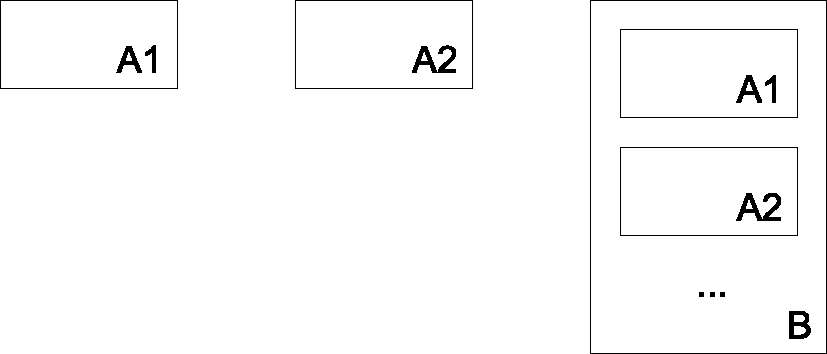
\includegraphics[width=7cm]{Figures/heritage1}
\end{center}
%--------------------------------------------------------------------
\subsection{Classes virtuelles}\index{classes!virtuelles}

On peut trouver des cas o� une classe d�rive indirectement plusieurs fois d'une classe de base.

Exemple :    
\begin{cpp}
class A { ... };

class B1 : public A { ... };
class B2 : public A { ... };

class C  : public B1, public B2 { ... };
\end{cpp}

On se retrouve alors avec l'objet de la classe �C� contenant deux sous-objets de la classe �A�. 

\begin{center}
    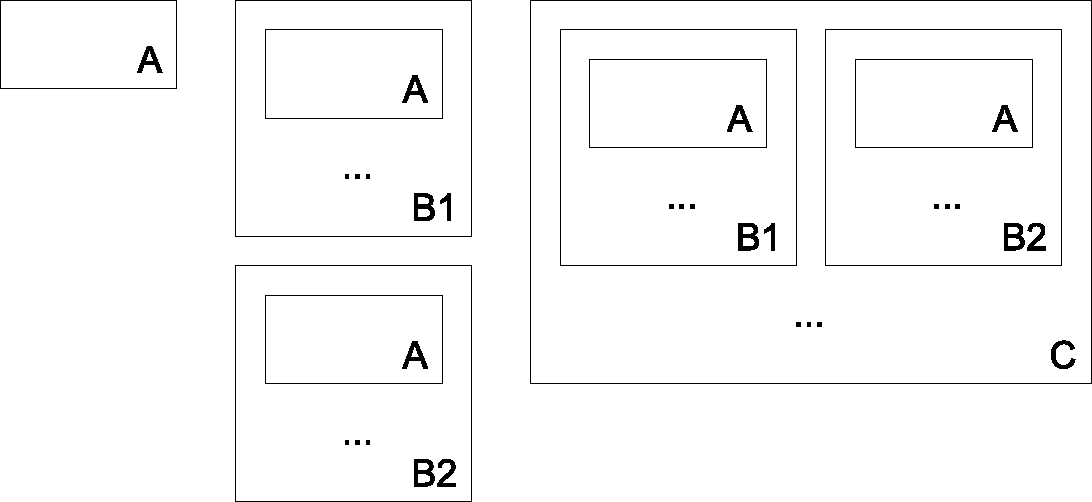
\includegraphics[width=9cm]{Figures/heritage2}
\end{center}

Si cet effet est ind�sirable, pour lever des ambigu�t�s, pour r�soudre les conflits et �conomiser la place m�moire, il suffit de d�clarer les classes �B1� et �B2� comme virtuelles:
\begin{cpp}
class A { ... };

class B1 : virtual public A { ... };
class B2 : virtual public A { ... };

class C  : public B1, public B2 { ... };
\end{cpp}

Un objet de la classe �C� poss�dera ainsi en un seul exemplaire les membres de la classe �A�.

\begin{center}
    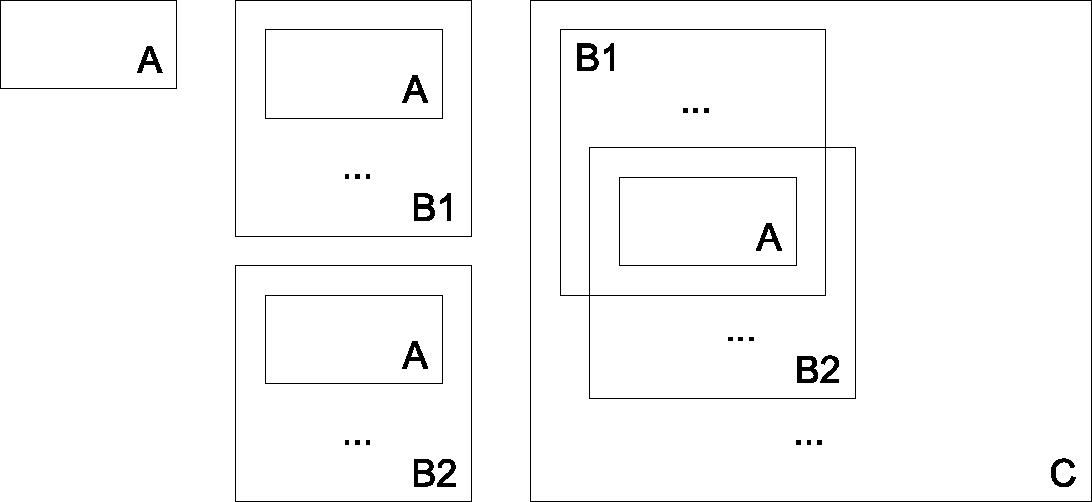
\includegraphics[width=9cm]{Figures/heritage3}
\end{center}


%%%%%%%%%%%%%%%%%%%%%%%%%%%%%%%%%%%%%%%%%%%%%%%%%%%%%%%%%%%%%%%%%%%%%
\section{Classes g�n�riques}\index{classes!g�n�riques}\index{template}

Il s'agit ici de classes param�tr�es par un ou plusieurs types. La d�claration d'une telle classe est pr�c�d�e du mot cl� �template� suivi des param�tres entre chevrons.

\begin{cppsyntaxe}
template < class e1,class e2,...,class en > class nom_de_la_classe {...};
\end{cppsyntaxe}

Les param�tres peuvent �tre un type de base (�int�, �double�, ...) ou un identificateur de classe. 

\begin{cpp}
template < class element > class Couple {...}; // couple de 2 �l�ments de m�me type

template < class element, int dim > class Tableau {...};    // tableau d'�l�ments de taille dim
\end{cpp}

On fait pr�c�der l'implantation d'une m�thode par �template < class e1,class e2,...,class en >� et, de plus, la m�thode est pr�fix�e par le nom de la classe rappelant le param�trage.

\begin{cppsyntaxe}
template < class e1,class e2,...,class en > 
    type_de_la_m�thode nom_de_la_classe<e1,e2,...,en>::nom_de_la_m�thode(arguments)  {
    ...
}
\end{cppsyntaxe}

Par exemple, on veut se fabriquer une classe \og{}Couple\fg{} comme �tant un couple d'�l�ments de type quelconque, pour pouvoir ensuite utiliser des couples d'entiers, de r�els, de complexes, d'individus, \etc

D�claration de la classe :

\begin{cpp}
template <class element> class Couple {
private    :
    element x,y;
public :
    void afficher(void);
    void acquerir(void);
};
\end{cpp}

Implantation des m�thodes de la classe :  

\begin{cpp}
template <class element> void Couple<element>::afficher(void) { 
    cout<<"couple  ="<<x<<"  "<<y<<endl;
};

template <class element> void Couple<element>::acquerir(void) {
    cout<<"entrer les �l�ments du couple ";
    cin>>x;
    cin>>y;
};
\end{cpp}

Utilisation :     

\begin{cpp}
int main() {
    Couple<int> a; // couple d'entiers
    a.acquerir();
    a.afficher();
    Couple<double> b; // couple de r�els
    b.acquerir();
    b.afficher();
    Couple<Complexe> c; // couple de complexes; la classe complexe et les op�rateurs
    c.acquerir();           // surcharg�s << et >> �tant d�finis par ailleurs
    c.afficher();        

    Couple<Complexe> t[10]; // t est un tableau de 10 couples de complexes
}
\end{cpp}

\begin{remark}
Dans le cas de classes param�tr�es, la seule inclusion �#include "nom_de_la_classe.h"� dans le fichier utilisateur peut conduire � des erreurs d'�dition de liens si l'implantation des m�thodes est ext�rieure dans un fichier �nom_de_la_classe.cpp�. Certains compilateurs n�cessitent �#include "nom_de_la_classe.cpp"� dans le fichier utilisateur.
\end{remark}

%%%%%%%%%%%%%%%%%%%%%%%%%%%%%%%%%%%%%%%%%%%%%%%%%%%%%%%%%%%%%%%%%%%%%
\section{Gestion des exceptions}\index{erreurs}\index{exceptions}

La gestion des exceptions propos�e par C++ est effectu�e � l'aide des mots cl�s �throw�, �catch� et �try�. \index{throw}\index{catch}\index{try}

Une exception peut �tre d'un type pr�-d�fini (entier ou cha�ne de caract�res, par exemple) ou une instance d'une classe d�finie par le programmeur.

Dans un bloc rep�r� par �try�, une exception est soulev�e � l'aide de �throw� et captur�e par �catch�.

\begin{cppsyntaxe}
try {
    // bloc d'instruction comportant des  throw  exception
    // ou des appels de fonctions comportant des throw  exception
}
catch (type_1 exception) {
    // traitement de l'exception
}
...
catch (type_n exception) {
    // traitement de l'exception
}
\end{cppsyntaxe}

L'exception soulev�e sera captur�e par le premier catch comportant un type compatible. 

Si aucun type n'est compatible, l'exception sera captur�e par une fonction �unexpected()� qui, par d�faut, fait appel � �abort()�.\index{unexpected}\index{abort}

L'ellipse �catch(...)� capture tous les types d'exception.\medskip

Lors d'appels imbriqu�s de fonctions, une exception est d'abord trait�e par la fonction la plus profonde. Si elle ne peut �tre captur�e par cette fonction, elle est retourn�e � la fonction appelant.

Lorsque une exception est d�clench�e, les objets cr��s dans le bloc �try� sont d�truits.\medskip

    
On peut pr�ciser les prototypes des fonctions en ajoutant avec �throw� les types d'exceptions qu'elles peuvent soulever : 
\begin{cppsyntaxe}
type nom_de_fonction(param�tres) throw (types exceptions) ;
\end{cppsyntaxe}

Exemple :    
\begin{cpp}

typedef  int  tableau[10];

void  fonction_exemple_exagere (tableau t, int i, double x) throw(int, string);
// cette fonction peut soulever des exceptions de type entier ou cha�ne de caract�res
// range la partie enti�re de x dans t[i]

int main() {
    tableau  a;
    int  k;
    double   r;
    try  {
        cout<<"taper l'indice : ";
        cin>>k;
        cout<<"taper la valeur : ";
        cin>>r;
        fonction_exemple_exagere(a,k,r);
    }
    catch (string) {
        cout << "avertissement :  " << e ;
    }
    catch (int e) {
        switch (e) {
            case 0: {
                cout <<"d�bordement d'indice bas " << i ;
                break;
            }
            case 1: {
                cout <<"d�bordement d'indice haut "<< i ;
                break;
            }
        }
        exit(1);
    }
    catch (double  e) {
        cout<<"valeur trop grande : "<<r ;
        exit(2);
    }
    catch (...) {
        cout << "exception non catalogu�e !" ;
        exit(3);
    }
    return 0;
}

void  fonction_exemple_exagere (tableau t, int i, double x) {
    if (i<0) 
        throw 0;
    if (i>9) 
        throw 1;
    if (abs(x)>=32767) {
        throw x ;
    };
    t[i]=abs(x);
    if ((i==0)||(i==9)) {
        throw "extr�mit� du tableau";
    };
    throw "tout est conforme ";
}
\end{cpp}


%%%%%%%%%%%%%%%%%%%%%%%%%%%%%%%%%%%%%%%%%%%%%%%%%%%%%%%%%%%%%%%%%%%%%
\chapter{Biblioth�ques standards du C++}\label{chap:Std_C++}

Ce chapitre pr�sente une s�lection des possibilit�s offertes par la biblioth�que standard du C++.

%%%%%%%%%%%%%%%%%%%%%%%%%%%%%%%%%%%%%%%%%%%%%%%%%%%%%%%%%%%%%%%%%%%%%
\section{Entr�es/sorties standards}\index{entr�es/sorties}\index{iostream}\index{std}
    
%--------------------------------------------------------------------
\subsection{Entr�es/sorties format�es}
\index{entr�es/sorties!format�es}\index{iostream}\index{std}


La biblioth�que �iostream� (incluse par �#include <iostream>�) d�finit de nouveaux classes et op�rateurs d'entr�es-sorties sur les types standards\footnote{Avant que le C++ ne soit normalis�, \lstinline�<iostream.h>� �tait le seul fichier d'en-t�te existant livr� avec les compilateurs de l'�poque. La normalisation ISO du C++ en 1998 a d�fini que \lstinline�<iostream>� serait l'en-t�te standard pour les entr�es-sorties. L'absence de \lstinline�.h� dans son nom indique qu'il s'agit d�sormais d'un en-t�te standard, et donc que toutes ses d�finitions font partie de l'espace de nom standard \lstinline�std�. Il est en de m�me avec tous les fichiers d'en-t�te standards en C++.}.\medskip

Les entr�es-sorties sont support�es par les classes �istream� (flot d'entr�e), �ostream� (flot de sortie) et �iostream� (flot d'entr�e-sortie, classe d�riv�e des deux pr�c�dentes).\index{istream}\index{ostream}\index{iostream}


Les variables et constantes suivantes sont �galement d�finies :
\begin{itemize}
    \item \lstinline�cin� objet de type \lstinline�istream�  reli� � l'entr�e standard (le clavier par d�faut);\index{cin}
    \item \lstinline�cout� objet de type \lstinline�ostream� reli� � la sortie standard (l'�cran par d�faut);\index{cout}
    \item \lstinline�endl� pour passer � la ligne suivante.\index{endl}
\end{itemize}

Les sorties se font par l'op�rateur �<<� :\index{op�rateurs!de flots}

\begin{cppsyntaxe}
ostream& operator<<(type x);          
\end{cppsyntaxe}

Par exemple:
\begin{cpp}
#include <iostream> 
using namespace std;

int main() 
{
    cout << "Hello world !" << endl;
    return 0;
}
\end{cpp}

ou :
\begin{cpp}
#include <iostream> 

int main()
{
    std::cout << "Hello world !" << std::endl;
    return 0;
}
\end{cpp}

ou encore :
\begin{cpp}
#include <iostream> 
using std::cout;
using std::endl;

int main() 
{
    cout << "Hello world !" << endl;
    return 0;
}
\end{cpp}

Les entr�es se font par l'op�rateur �>>� :

\begin{cppsyntaxe}
istream& operator>>(type & x);      
\end{cppsyntaxe}

Par exemple:
\begin{cpp}
#include <iostream>
using namespace std;

int main()
{
    double x,y;
    cout<<"entrer x ";  
    cin>>x;
    cout<<"entrer y ";
    cin>>y;

    cout<<" x = ";
    cout<<x;
    cout<<" y = ";
    cout<<y;
    cout<<endl;
    return 0;
}
\end{cpp}

On peut regrouper plusieurs expressions d'entr�es-sorties en une seule:
\begin{cpp}
#include <iostream>
using namespace std;

int main()
{
    double x,y;
    cout<<"entrer x et y ";  
    cin>>x>>y;

    cout<<" x = "<< x <<" y = "<< y <<endl;
    return 0;
}
\end{cpp}

Pour lire un seul caract�re, on utilise la m�thode �get� :
\begin{cpp}
#include <iostream>
using namespace std;

int main()
{
    char c;
    
    c = cin.get();

    cout<<" c = "<< c <<endl;
    
    return 0;
}
\end{cpp}



Si l'on souhaite prendre en compte tous les caract�res d'une cha�ne et ne pas �liminer les blancs, tabulations, retours � la ligne et caract�res de fin de fichier, on peut utiliser la m�thode �getline� :
\begin{cpp}
#include <iostream>
using namespace std;

int main()
{
    char buffer[256];
    
    cin.getline(buffer,256);

    cout<<" buffer = "<< buffer <<endl;
    
    return 0;
}
\end{cpp}

% Donner un exemple !

%Remarque :  
%
%        istream&  read ( char * s , int  n )
%        int  gcout ( void )
%        int  peek ( void )
%        istream&  ignore ( int  n = 1 , int delim = EOF )
%        istream&  putback ( char c )
%
%        ostream&  put ( char c )
%        ostream&  write ( const char * s , int  n )
%        ostream&  flush ( void )

%--------------------------------------------------------------------
\subsection{Manipulateurs}
\index{manipulateurs}\index{iomanip}

La biblioth�que <iomanip> fournit des outils de formatage appel�s manipulateurs pour mettre en forme les donn�es lors de l'affichage � l'�cran :
\begin{itemize}
    \item \lstinline�setw(n)� fixe la largeur de la zone d'affichage � n caract�res,\index{setw}
    \item \lstinline�setprecision(n)�    fixe le nombre de chiffres � afficher d'un nombre r�el,\index{setprecision}
    \item \lstinline�setfill('X')� remplit la zone libre par des caract�res X,\index{setfill}
    \item \lstinline�hex� pour lire ou afficher le prochain nombre en hexad�cimal,\index{hex}
    \item \lstinline�oct�    pour lire ou afficher le prochain nombre en octal,\index{oct}\medskip
\end{itemize}

Exemple :
\begin{cpp}
#include <iostream>
#include <iomanip>
using namespace std;

void main( void )
{
    int n;
    double a;
    n=86;
    a=-13.141592;
    
    cout<<"Affichage normal  : "<<n<<endl;
    cout<<"Affichage formate : "<<setw(10)<<n<<endl;
    cout<<"Affichage normal  : "<<a<<endl;
    cout<<"Affichage formate : "<<setprecision(3)<<a<<endl;
    cout<<"Affichage normal  : "<<setw(10)<<"ENSMM"<<"Besancon"<<endl;
    cout<<"Affichage formate : "<<setw(10)<<setiosflags(ios::left)<<"ENSMM"
    cout<<"Besancon"<<endl;
}
\end{cpp}

R�sultat produit � l'�cran :
\begin{console}
Affichage normal  : 86
Affichage formate :         86
Affichage normal  : -13.1416
Affichage formate : -13.1
Affichage normal  :      ENSMMBesancon
Affichage formate : ENSMM     Besancon
\end{console}

Ces manipulateurs font appels aux m�thodes �fill()�, �width()�, �precision()� de la classe �ios�. On peut donc aussi �crire :
\begin{cpp}
cout.fill('_');
cout.width(10);
cout.precision(3);
cout<<a<<endl;
\end{cpp}

Ce qui donne :
\begin{console}
_____-13.1
\end{console}


%%%%%%%%%%%%%%%%%%%%%%%%%%%%%%%%%%%%%%%%%%%%%%%%%%%%%%%%%%%%%%%%%%%%%
\section{Entr�es/sorties sur les fichiers}
\index{entr�es/sorties!fichiers}\index{fstream}\index{ifstream}\index{ofstream}


La biblioth�que �<fstream>� d�finit des classes permettant de lire et d'�crire dans des fichiers format�s : 
\begin{itemize}
    \item \lstinline�ifstream� classe des fichiers ouverts en lecture, classe d�riv�e de �istream�;
    \item \lstinline�ofstream� classe des fichiers ouverts en �criture, classe d�riv�e de �ostream�;
    \item \lstinline�fstream� classe des fichiers ouverts en lecture-�criture, classe d�riv�e de \lstinline�iostream�.\medskip
\end{itemize}

Ces classes de flots fichiers h�ritent des m�thodes de leurs classes m�res auxquelles s'ajoutent quelques m�thodes suivantes particuli�res.\medskip

L'ouverture d'un fichier s'effectue implicitement lors de sa d�claration par la m�thode constructeur ou explicitement par la m�thode �open()�.

\begin{cppsyntaxe}
/* constructeurs sans ouverture */        
ifstream::ifstream(void);
ofstream::ofstream(void);
fstream::fstream(void);

/* constructeurs avec ouverture */    
ifstream::ifstream(const char* nom,int mode=ios::in,int prot=filebuf::openprot);
ofstream::ofstream(const char* nom,int mode=ios::out,int prot=filebuf::openprot);
fstream::fstream(const char* nom,int mode,int prot filebuf::openprot);

/* ouverture explicite */
void ifstream::open(const char* nom,int mode=ios::in,int prot=filebuf::openprot);
void ofstream::open(const char* nom,int mode=ios::out,int prot=filebuf::openprot);
void fstream::open(const char* nom,int mode,int prot filebuf::openprot);
\end{cppsyntaxe}

La valeur de protection par d�faut �openprot� repr�sente le droit de lecture-�criture pour le propri�taire du fichier et le droit de lecture pour tous.

La valeur du mode est � choisir parmi les valeurs : �ios::in�, �ios::out�, �ios::app�, �ios::trunc�, �ios::ate�, �ios::nocreate� ou �ios::noreplace�.

Le mode peut �tre une concat�nation de plusieurs valeurs, par exemple : �ios::in | ios::out | ios::noreplace�\medskip 


Les autres m�thodes sont :
\begin{cppsyntaxe}
void      close(void);        
streampos tellg(void); //  retourne la position courante dans le fichier
ifstream& seekg(streampos p); // d�placement absolu
ifstream& seekg(streampos dep,ios::seek_dir pos);    // d�placement relatif
// le param�tre pos peut �tre ios::beg, ios::cur ou ios::end
\end{cppsyntaxe}

Comme les classes des biblioth�ques d'entr�es-sorties, les classes de flots fichiers poss�dent un ensemble de variables indicatrices de l'�tat d'un flot. Cet �tat peut �tre consult� en appelant les m�thodes suivantes :
\begin{cppsyntaxe}
int eof(void);
int bad(void);
int fail(void);
int good(void);
int rdstate(void);
void clear(int i=0);
\end{cppsyntaxe}

% Donner des exemples !!!


%%%%%%%%%%%%%%%%%%%%%%%%%%%%%%%%%%%%%%%%%%%%%%%%%%%%%%%%%%%%%%%%%%%%%
\section{Les classes conteneurs de la STL}
\index{STL}\index{Standart Template Library}\index{conteneurs}

La biblioth�que g�n�rique standard (Standart Template Library) est une biblioth�que C++, normalis�e par l'ISO (document ISO/CEI 14882). L'une des implantations les plus diffus�es de la STL a �t� d�velopp�e historiquement par Hewlett-Packard, puis par Silicon Graphics\footnote{Une documentation compl�te est disponible sur le site de Silicon Graphics~: http://www.sgi.com/tech/stl/}. 

%La STL est constitu�e de classes g�n�riques et de sous-programmes permettant de r�aliser rapidement les structures de donn�es classiques et les algorithmes associ�s.

La STL fournit un ensembles de classes g�n�riques, appel�es conteneurs, permettant de g�n�rer les structures de donn�es les plus r�pandues telles que les tableaux, les listes (cha�n�es), les tableaux associatifs, \etc Il existe deux cat�gories de conteneurs~: les conteneurs s�quentiels et les conteneurs associatifs. 

%--------------------------------------------------------------------
\subsection{Les conteneurs s�quentiels}

Les �l�ments d'un conteneur s�quentiel sont stock�s selon un ordre~: le deuxi�me suit le premier, le troisi�me suit le deuxi�me, \etc On peut parcourir le conteneur selon cet ordre (du premier au dernier). Enfin, quand on ins�re ou quand on supprime un �l�ment, on le fait � une place qu'on a explicitement choisie. 

Les trois principaux conteneurs s�quentiels sont~: les tableaux ou collections statiques (classe �vector�), les listes cha�n�es (classe �list�) et les files (classe �deque�). Ces trois classes ont une interface proche mais se distinguent par des implantations diff�rentes.\index{vector}\index{list}\index{deque}

\begin{center}
    \begin{tabular}{|l|c|c|c|}
    \hline
        &  \lstinline�vector�    &  \lstinline�deque� & \lstinline�list� \\
        \hline
        Acc�s � un �l�ment  & O(1)    & O(1)    & O(N) \\
        \hline
    Insertion/suppression d'un �l�ment en queue & O(1)    & O(1) & O(1) \\
        \hline
    Insertion/suppression d'un �l�ment en t�te & O(N) & O(1) & O(1) \\
        \hline
    Insertion/suppression d'un �l�ment au milieu & O(N) & O(N) & O(1)\\
        \hline
    \end{tabular}
\end{center}

Les biblioth�ques � inclure portent le nom des conteneurs (�<vector>�, �<list>� et �<deque>�). Toutes les classes sont d�finies dans l'espace de nom �std�.

\subsubsection{M�thodes communes}

Les trois conteneurs �vector�, �deque� et �list� ont un certain nombre de m�thodes communes (�operator=�, �size�, �empty�, �clear�, �operator==�, �operator<�, �back�, �push_pack�, �pop_back�, �begin�, �end�, �insert�, �erase�) qui sont d�taill�es dans les exemples suivants.

\paragraph{Construction}~

\begin{cpp}
list<int>      L;        // La liste L est vide

list<int>      A(10);    // La liste A contient 10 entiers non initialis�s
vector<double> V(20);    // Le vecteur V contient 20 r�els non initialis�s

list<int>      B(10,0);  // La liste B contient 10 entiers initialis�s � 0
deque<int>     D(20,-1); // La file D contient 20 entiers initialis�s � -1
\end{cpp}

Dans les exemples suivants, �X� et �Y� d�signeront arbitrairement des conteneurs �vector�, �deque� ou �list�.

\paragraph{Affectation et recopie}~

Les op�rateurs d'affection et de recopie (passage par valeur) sont d�finis et utilisables directement.
\begin{cpp}
X=Y; // copie effective des �l�ments de X dans Y
     // X et Y appartenant � la m�me classe
\end{cpp}

\paragraph{Nombre d'�l�ments (dimension)}~

\begin{cpp}
int N=X.size();    // N re�oit la dimension de X
if (X.empty()) ... // Teste si X est vide
\end{cpp}

\paragraph{Vider un conteneur}~

\begin{cpp}
X.clear(); // X.size() vaut maintenant 0
\end{cpp}

\paragraph{Comparaison entre conteneurs}~

Ces op�rateurs supposent que des op�rateurs correspondants (�==�, �<�, \etc) soient d�finis sur les �l�ments.
\begin{cpp}
if (X==Y) ... // vrai si X et Y sont identiques (m�me �l�ments, m�me taille)
if (X<Y) ...  // comparaison lexicographique entre X et Y
\end{cpp}

\paragraph{Ajout/suppression en queue}~

Les trois conteneurs disposent de m�thodes d'acc�s, d'ajout et de suppression du dernier �l�ment en �O(1)�.

\begin{cpp}
int x=X.back();  // x re�oit la valeur du dernier �l�ment de X
X.push_back(45); // ajoute un �l�ment de valeur 45 � la fin X
X.pop_back();    // supprime le dernier �l�ment
\end{cpp}

\paragraph{Acc�s aux �l�ments, notion d'it�rateur}~\index{it�rateurs}

Pour tous les conteneurs, l'acc�s aux �l�ments peut se faire par l'interm�diaire d'un it�rateur. Un it�rateur est un objet d�fini par la classe conteneur (d'o� la d�claration �list<int>::iterator� par exemple) qui se comporte comme un pointeur sur les �l�ments du conteneur. Les deux exemples qui suivent sont valables �galement pour �vector� et �deque�.
\begin{cpp}
list<int>::iterator il; // it�rateur sur les �l�ments d'une liste d'entiers
il=L.begin();           // il pointe sur le premier �l�ment de L
*il=35;                 // affecte la valeur 35 au premier �l�ment de L
il++;                   // avance d'un �l�ment
cout<<*il;              // affiche la valeur du deuxi�me �l�ment de L

il=L.begin();           // il pointe sur le premier �l�ment de L
while (il!=L.end()) {    // tant qu'il y a encore des �l�ments
    cout<<*il;          // affiche l'�l�ment point� par il
    il++;               // avance d'un �l�ment
}
\end{cpp}

\paragraph{Insertion/suppression d'un �l�ment}~

\begin{cpp}
L.insert(il,5);   // ins�re un �l�ment devant l'�l�ment point� par il
V.erase(il);      // supprime l'�l�ment point� par il
                  // apr�s cet appel il n'est plus valide
il=V.erase(il);   // supprime l'�l�ment point� par il et il pointe sur
                 // l'�l�ment suivant
\end{cpp}

\subsubsection{M�thodes du conteneur vector}

Le conteneur �vector� correspond au concept de tableau ou collection statique.

\paragraph{Acc�s direct aux �l�ments}~

Dans un conteneur �vector�, l'acc�s aux �l�ments (et leur modification) est direct avec l'op�rateur �[]�. Les indices courent de �0� � �V.size()-1�.
\begin{cpp}
for (int i=0 ;i<V.size();i++)
    V[i]=2*V[i];         // double toutes les valeurs
\end{cpp}

\paragraph{Ajout/suppression en queue}~

Comme �list� et �deque�, le conteneur �vector� dispose des m�thodes d'acc�s, d'ajout et de suppression du dernier �l�ment en �O(1)�. Si la dimension du conteneur diminue, les espaces m�moires en surplus sont conserv�s. Si la dimension du conteneur augmente et d�passe la taille maximum qu'il a atteint dans le pass�, le conteneur proc�de � une r�allocation en m�moire (op�ration tr�s lente en �O(N)�).

\paragraph{Modification de la dimension}~

On peut changer � tout moment la dimension d'un conteneur �vector� (ce qui provoque une r�allocation en m�moire).
\begin{cpp}
vector<int> V;  // V est cr�� vide (dimension nulle)
V.resize(10);   // V est maintenant de taille 10
V.resize(20,4); // V contient maintenant 20 entiers initialis�s � 4
\end{cpp}

\paragraph{Utilisation des m�thodes communes n�cessitant un it�rateur}~

Pour obtenir de mani�re directe un it�rateur sur un �l�ment du conteneur, on utilise l'op�rateur �&�.

\begin{cpp}
vector<int> V(10,3); // V=<3,3,3,3,3,3,3,3,3> 
V.insert(&V[3],7);   // V=<3,3,3,7,3,3,3,3,3,3>
V.erase(&V[2],7);    // V=<3,3,7,3,3,3,3,3,3>
\end{cpp}

\subsubsection{M�thodes du conteneur deque}

Le conteneur �deque� dispose des m�mes fonctionnalit�s que �vector�
mais il permet en plus l'acc�s, l'ajout et la suppression en t�te en �O(1)� avec les m�thodes~: �front�, �push_front� et �pop_front�. Naturellement,
les autres op�rations sur �deque� sont l�g�rement plus lentes que sur
�vector�.

\begin{cpp}
deque<int> D;
D.push_front(45); // ajoute un �l�ment de valeur 45 en t�te D
D.pop_front();    // supprime le premier �l�ment
int x=D.front();    // x re�oit la valeur du premier �l�ment de D
\end{cpp}

\subsubsection{M�thodes du conteneur list}

Le conteneur �list� est une liste doublement cha�n�e. L'acc�s direct n'est
pas possible (avec l'op�rateur �[]�), il faut obligatoirement utiliser un it�rateur.

\paragraph{Acc�s/ajout/suppression d'�l�ment}~

Le conteneur �list� dispose des m�thodes d'acc�s, d'ajout et de
suppression en t�te et en queue~: �front�, �back�,
�push_front�, �pop_front�, �push_back�,
�pop_back�.

\paragraph{Autres m�thodes}~

\begin{cpp}
L.sort();    // trie la liste L
L.merge(B);  // fusion de deux listes ordonn�es
L.remove(0); // retire tous les �l�ments nuls de L
L.unique();  // L n'a plus de doublons !

L.remove_if(Pair); // retire tous les �l�ments pairs de L
// suppose qu'une fonction Pair est d�finie, par exemple :
// bool Pair(int n)
// { return(n%2); }
\end{cpp}

\subsubsection{Algorithmes g�n�riques}

Les algorithmes g�n�riques sont des sous-programmes qui manipulent un conteneur quelle que soit sa classe. Ils sont d�finis dans la biblioth�que �<algorithm>�. Ces algorithmes supposent que les op�rateurs �==� et �<� sont d�finis sur les �l�ments. Les quelques exemples qui suivent sont valables  pour �vector�, �deque� et �list�.

\paragraph{Algorithmes de recherche}~

\begin{cpp}
list<int>::iterator il;
il=find(L.begin(),L.end(),10); // renvoie un it�rateur sur le premier
                               // �l�ment �gal � 10 si il existe et
                               // l'it�rateur L.end() sinon
il=find_if(L.begin(),L.end(),Pair()); // Trouve le premier �l�ment pair
\end{cpp}

\paragraph{Algorithme de recherche dichotomique (pour un conteneur tri�)}~

\begin{cpp}
list<int>::iterator il;
il=binary_search(L.begin(),L.end(),10);
\end{cpp}

\paragraph{Algorithmes de recherche de maximum ou de minimum}~

\begin{cpp}
list<int>::iterator il;
il=min_element(L.begin(),L.end());
il=max_element(L.begin(),L.end());
\end{cpp}

\paragraph{Algorithme de tri}~

\begin{cpp}
sort(V.begin(),V.end());
\end{cpp}

\subsection{Les conteneurs associatifs}

Les conteneurs associatifs ont pour vocation de retrouver une information non plus en fonction de sa place dans le conteneur mais en fonction de sa valeur ou d'un partie de sa valeur appel�e cl�. Par exemple, un dictionnaire peut �tre mod�lis� par un conteneur associatif contenant des articles dont la cl� d'acc�s serait d�finie par le mot correspondant � l'article. 

Les deux conteneurs associatifs les plus importants sont �map� et �multimap�.\index{map}\index{multimap}


%%%%%%%%%%%%%%%%%%%%%%%%%%%%%%%%%%%%%%%%%%%%%%%%%%%%%%%%%%%%%%%%%%%%%
\section{La classe string}
\index{cha�nes de caract�res}\index{string}\index{types!cha�nes de caract�res}

La classe �string� de la biblioth�que �<string>� offre un cadre pratique pour manipuler les cha�nes de caract�res en C++. Les op�rateurs usuels (affectation �=�, concat�nation avec �+�, \etc) ainsi que les entr�es-sorties standards (�cout�, �cin�) sont utilisables directement.

Le petit programme ci-dessous illustre la facilit� d'utilisation de cette classe~:
\begin{cpp}
string A,B(", ca va ?");
A="bonjour";
A=A+" antoine";
A=A+B;
A[0]='B';
B=A;
cout<<A<<endl;
if (A==B) cout<<"A est identique � B"<<endl;
\end{cpp}

Le code suivant d�crit les principales m�thodes de cette classe sous la forme
d'une d�finition de classe simplifi�e (la d�finition r�elle utilise la classe g�n�rique �basic_string� et est peu lisible.

\begin{cppsyntaxe}
class string {
private:
    ...
public:
    /// construit moi-m�me avec une cha�ne de caract�re entre 
    /// guillemets
    string(char * ch="");
    
    /// constructeur de recopie
    string(const string & s);
    
    /// lib�re la m�moire
    ~string();

    /// moi-m�me re�oit s
    void operator=(const string & s);
    
    /// moi-m�me re�oit une cha�ne de caract�re entre guillemets
    void operator=(char * ch);
    
    /// renvoie vrai si moi-m�me est avant s dans l'ordre 
    /// alphab�tique
    bool operator<(string s);
    
    /// renvoie vrai si moi-m�me et s sont identiques
    bool operator==(string s);
    
    /// renvoie moi-m�me suivi de la cha�ne s (concat�nation)
    string operator+(string s);

    /// renvoie le i�me caract�re de moi-m�me
    char & operator[](int i);

    /// renvoie la taille de moi-m�me
    int size(void);
    
    /// renvoie vrai si moi-m�me est vide
    bool empty(void);

    /// renvoie la position de la premi�re occurence de s 
    /// dans moi-m�me, si s n'est pas dans moi-m�me alors le 
    /// r�sultat est <0 ou >size()
    int find(string s);

    /// insert s � la i�me position dans moi-m�me
    void insert(int i,string s);
    
    /// supprime n caract�res de moi-m�me � partir du i�me caract�re
    void erase(int i,int n);
    
    /// remplace n caract�res de moi-m�me � partir du i�me caract�re
    /// par ceux de s
    void replace(int i,int n,string s);
    
    /// renvoie une sous-cha�ne de moi-m�me de taille n � partir 
    /// du i�me caract�re
    string substr(int i,int n);

    /// renvoie un pointeur sur un tableau de caract�res contenant
    /// la cha�ne stock� par moi-m�me
    char * c_str(void);
};
\end{cppsyntaxe}

%%%%%%%%%%%%%%%%%%%%%%%%%%%%%%%%%%%%%%%%%%%%%%%%%%%%%%%%%%%%%%%%%%%%%
\section{Lecture et �criture de donn�es (r�els, entiers, \etc) dans une cha�ne de caract�res}

Les classes �ostringstream� et �istringstream� de la biblioth�que �<sstream>� permettent de convertir des valeurs num�riques en cha�nes de caract�res � l'aide des op�rateurs de flot.\index{ostringstream}\index{istringstream}\index{sstream}

Exemple de conversion d'un entier en cha�ne de caract�res :
\begin{cpp}
int n=13;
string s;
ostringstream os;
os<<n;
s=os.str();  // s re�oit la cha�ne "13"
\end{cpp}

Pour lire des donn�es contenues dans une cha�ne, on proc�de de la mani�re suivante :
\begin{cpp}
int n;
string s="13";
istringstream is(s);
is>>n;       // n prends la valeur 13
\end{cpp}

%%%%%%%%%%%%%%%%%%%%%%%%%%%%%%%%%%%%%%%%%%%%%%%%%%%%%%%%%%%%%%%%%%%%%
\section{Classe complex}
\index{nombres complexes}\index{complex}\index{types!complexes}


La biblioth�que �complex� d�finit une classe g�n�rique permettant de manipuler des nombres complexes de fa�on naturelle.
\begin{cpp}
#include <iostream>
#include <complex>
using namespace std;

int main() {
    complex<double> x,y,z(0,0);

    x=0.5+2i;

    y=complex<double>(5,7);

    z=x+exp(y*conj(y));

    cout<<x<<endl<<y<<endl<<z<<endl;

    return 0;
}
\end{cpp}

Un certain nombre de fonctions usuelles sont �galement propos�es (ou surcharg�es)  :  
�real�, �imag�, �abs�, �arg�, �norm�, �conj�, �polar�, �cos�, �cosh�, �exp�, �log�, �log10�, �pow�, �sin�, �sinh�, �sqrt�, �tan�, �tanh�.

\index{fonctions!complexes}\index{real}\index{imag}\index{abs}\index{arg}\index{norm}\index{conj}\index{polar}\index{abs}\index{exp}\index{log}\index{log10}\index{pow}\index{sqrt}\index{sin}\index{cos}\index{tan}\index{asin}\index{acos}\index{atan}\index{atan2}\index{sinh}\index{cosh}\index{tanh}




%----------------------------------------------------------------------------------------

\stopcontents[part] % Manually stop the 'part' table of contents here so the previous Part page table of contents doesn't list the following chapters

%----------------------------------------------------------------------------------------
%	BIBLIOGRAPHY
%----------------------------------------------------------------------------------------

%\chapterimage{} % Chapter heading image
%\chapterspaceabove{2.5cm} % Whitespace from the top of the page to the chapter title on chapter pages
%\chapterspacebelow{2cm} % Amount of vertical whitespace from the top margin to the start of the text on chapter pages
%
%%------------------------------------------------
%
%\chapter*{Bibliography}
%\markboth{\sffamily\normalsize\bfseries Bibliography}{\sffamily\normalsize\bfseries Bibliography} % Set the page headers to display a Bibliography chapter name
%\addcontentsline{toc}{chapter}{\textcolor{ocre}{Bibliography}} % Add a Bibliography heading to the table of contents
%
%\section*{Articles}
%\addcontentsline{toc}{section}{Articles} % Add the Articles subheading to the table of contents
%
%\printbibliography[heading=bibempty, type=article] % Output article bibliography entries
%
%\section*{Books}
%\addcontentsline{toc}{section}{Books} % Add the Books subheading to the table of contents
%
%\printbibliography[heading=bibempty, type=book] % Output book bibliography entries

%----------------------------------------------------------------------------------------
%	INDEX
%----------------------------------------------------------------------------------------

\chapterimage{orange1.jpg}

\cleardoublepage % Make sure the index starts on an odd (right side) page
\phantomsection
\addcontentsline{toc}{chapter}{\textcolor{ocre}{Index}} % Add an Index heading to the table of contents
\printindex % Output the index

%----------------------------------------------------------------------------------------
%	APPENDICES
%----------------------------------------------------------------------------------------

%\chapterimage{orange2.jpg} % Chapter heading image
%\chapterspaceabove{6.75cm} % Whitespace from the top of the page to the chapter title on chapter pages
%\chapterspacebelow{7.25cm} % Amount of vertical whitespace from the top margin to the start of the text on chapter pages
%
%\begin{appendices}
%
%\renewcommand{\chaptername}{Appendix} % Change the chapter name to Appendix, i.e. "Appendix A: Title", instead of "Chapter A: Title" in the headers
%
%%------------------------------------------------
%
%\chapter{Appendix Chapter Title}
%
%\section{Appendix Section Title}
%
%Lorem ipsum dolor sit amet, consectetur adipiscing elit. Aliquam auctor mi risus, quis tempor libero hendrerit at. Duis hendrerit placerat quam et semper. Nam ultricies metus vehicula arcu viverra, vel ullamcorper justo elementum. Pellentesque vel mi ac lectus cursus posuere et nec ex. Fusce quis mauris egestas lacus commodo venenatis. Ut at arcu lectus. Donec et urna nunc. Morbi eu nisl cursus sapien eleifend tincidunt quis quis est. Donec ut orci ex. Praesent ligula enim, ullamcorper non lorem a, ultrices volutpat dolor. Nullam at imperdiet urna. Pellentesque nec velit eget est euismod pretium.
%
%%------------------------------------------------
%
%\chapter{Appendix Chapter Title}
%
%\section{Appendix Section Title}
%
%Lorem ipsum dolor sit amet, consectetur adipiscing elit. Aliquam auctor mi risus, quis tempor libero hendrerit at. Duis hendrerit placerat quam et semper. Nam ultricies metus vehicula arcu viverra, vel ullamcorper justo elementum. Pellentesque vel mi ac lectus cursus posuere et nec ex. Fusce quis mauris egestas lacus commodo venenatis. Ut at arcu lectus. Donec et urna nunc. Morbi eu nisl cursus sapien eleifend tincidunt quis quis est. Donec ut orci ex. Praesent ligula enim, ullamcorper non lorem a, ultrices volutpat dolor. Nullam at imperdiet urna. Pellentesque nec velit eget est euismod pretium.
%
%%------------------------------------------------
%
%\end{appendices}

%----------------------------------------------------------------------------------------

\end{document}
